%!TEX root = ../../../adrien_gomar_phd.tex

\subsection{Convergence analysis}
\label{sub:dream_ls_conv_coeff}

The convergence of the steady computation using the Roe~2 space scheme
is reported in Fig.~\ref{fig:dream_ls_convergence_roe2}. The residuals
show a four order of magnitude decrease and the similarity
coefficients are stable starting at 500~iterations.
Therefore, according to \citet{Casey2000}, the
solution is considered to be converged.
\begin{figure}[htp]
  \centering
  \subfigure[residuals]{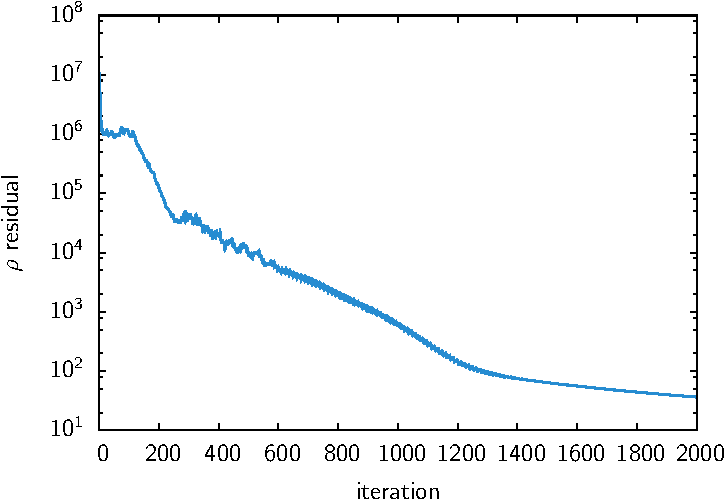
\includegraphics[width=.35\textwidth]{DREAM_LS_RESIDUALS_PPT.pdf}}
  \subfigure[$C_T$]{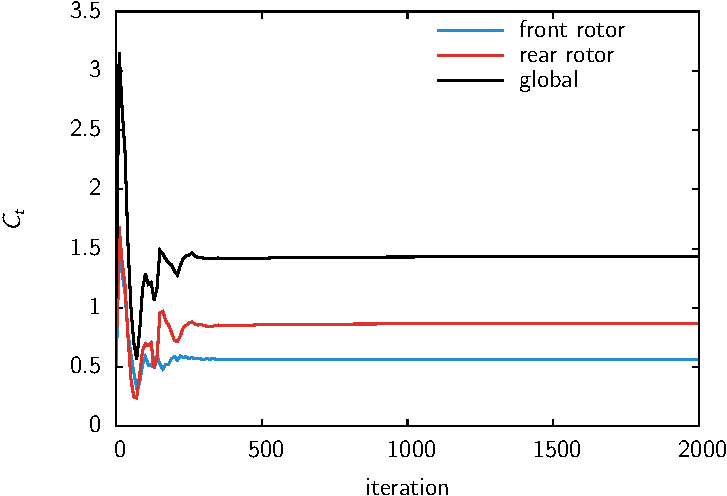
\includegraphics[width=.35\textwidth]{DREAM_LS_FORCES_CT_PPT.pdf}}
  \subfigure[$C_P$]{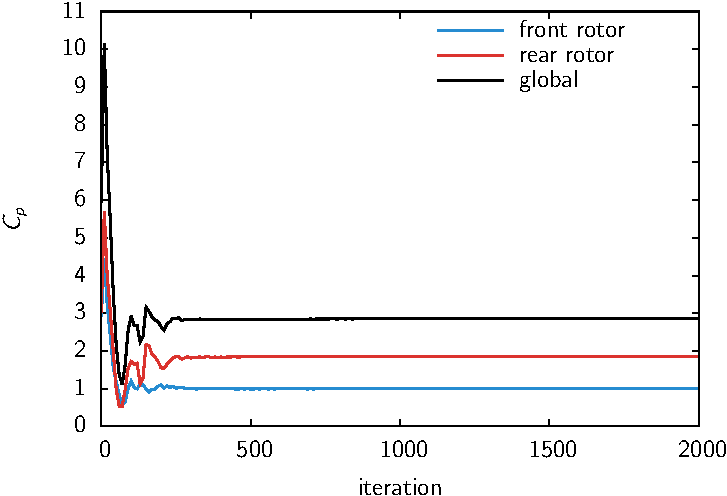
\includegraphics[width=.35\textwidth]{DREAM_LS_FORCES_CP_PPT.pdf}}
  \subfigure[$\eta$]{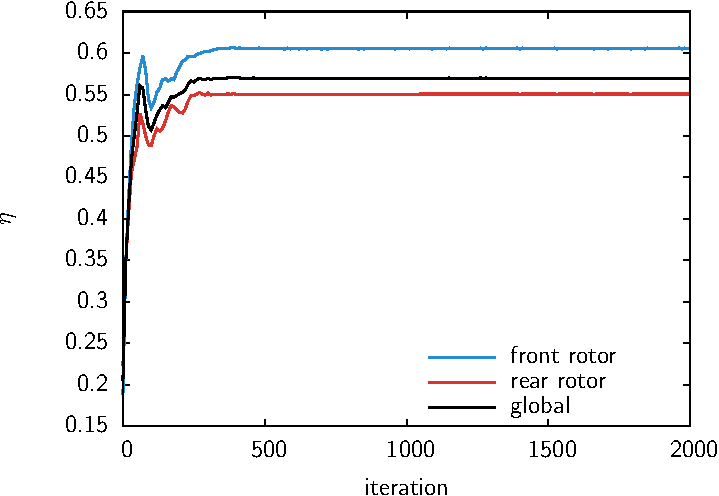
\includegraphics[width=.35\textwidth]{DREAM_LS_FORCES_ETA_PPT.pdf}}
  \caption{Low-speed isolated configuration: convergence of the Roe~2 steady
  computation.}
  \label{fig:dream_ls_convergence_roe2}
\end{figure}

\subsection{Similarity coefficients}
\label{sub:dream_ls_sim_coeff}

The similarity coefficients (defined in 
Sec.~\ref{sub:cror_similarity_coeff}) are post-processed 
and reported in Tab.~\ref{tab:dream_ls_sim_coeff}.
\begin{table}[htp]
  \ra{1.3} \centering
  \begin{tabular}{ccc|cccccc}
    \toprule
    $C_T$ & $C_P$ & $\eta$ & $C_{T_f}$ & $C_{P_f}$ & $\eta_f$ & $C_{T_r}$ & $C_{P_r}$ & $\eta_r$ \\
    \midrule
    1.1319 & 2.0927 & 0.5726 & 0.5637 & 0.9941 &  0.6002 & 0.5682 & 1.0986 &  0.5475 \\
    \bottomrule
  \end{tabular}
  \caption{Low-speed isolated configuration: similarity coefficients.}
  \label{tab:dream_ls_sim_coeff}
\end{table}
The results are consistent with the efficiency estimation given in 
Eq.~\eqref{eq:estimation_sim_coeff} for a propeller at take-off flight conditions.
In fact, each rotor of the CROR has an efficiency that is between $0.5$
and $0.6$. The advantage of the CROR is demonstrated here as the rear
rotor is able to retrieve an additional thrust coefficient of $0.5682$ yielding
a total of $1.1319$, while
the front rotor alone would only give $0.5637$.
The second rotor allows thus to more than double the total thrust of the engine.
However, the efficiency is affected compared to a single row 
propeller, as
it goes from $0.6002$ for the front rotor alone to $0.5726$ for the CROR.
Nevertheless, achieving such a level of thrust coefficient ($C_T = 1.1319$)
with an isolated
propeller would require a higher loading of the blades which is not
consistent with an increase of the efficiency, necessary to meet the ACARE goals.
Actually, this is another advantage 
of the CROR engine: two rotors are used to create the thrust which allows to
reduce the loading of each rotor compare to an isolated propeller,
allowing thus higher inflow Mach numbers. In fact, the rotation of the rotors is reduced 
to maintain a subsonic Mach number optimizing thus the efficiency
for a given level of thrust.


\subsection{One-dimensional results: radial profiles}
\label{sub:dream_ls_radial_profiles}

Radial profiles positioned at six locations upstream and downstream the rotors
are extracted and shown in Fig.~\ref{fig:dream_ls_position_radial}.
The absolute
Mach number, absolute flow angle, static pressure, 
stagnation pressure and stagnation temperature
are shown in Fig.~\ref{fig:dream_ls_radial_profiles}
against the radial position expressed
relative to the radius of the front rotor blade $R_f$.

The absolute Mach number, shown in 
Fig.~\ref{fig:dream_ls_radial_profiles_ma}, is increased by
the two rotors as it goes from the inflow condition value $M=0.2$
up to $M=0.4$. Note that above $R/R_f=1$, namely at the tip
of the front rotor blade, the Mach number
almost recovers the inflow condition. Moreover, it can be inferred from the
absolute Mach number radial evolution, that the stream tube is contracting which is consistent
with the observed acceleration of the fluid.

The pitch angle of the absolute velocity vector is shown in 
Fig.~\ref{fig:dream_ls_radial_profiles_alpha}. The front rotor
deviates the flow of almost $20^\circ$, justifying the need
for a second rotor. Between the fourth and the fifth extraction planes, namely
passing through the rear rotor, the flow is straighten up. Remember that 
the motivation for adding a second rotor to a propeller
was to recover the energy lost by the swirling flow
(recall Sec.~\ref{sub:cror_velocity_triangle}). This is observed in our simulations as
the deflection angle is now close to $0^\circ$ for $0.3 \leq R/R_f \leq 0.7$
in plane $P6$.
Below that, the deflection angle remains negative. In the tip vortex region
of the rear rotor, one can see the effect of the two tip vortices: between 
$0.8 \leq R/R_f \leq 0.9$, the front rotor tip vortex is seen as the 
deflection angle is positive while between $0.7 \leq R/R_f \leq 0.8$
the rear rotor is observed, 
which is consistent with the positive
peak observe near the blade tip region in planes $P3$ and $P4$.

The goal of a CROR is to create thrust through an acceleration of 
the flow rather than to produce static pressure as in a compressor stage.
This is highlighted in Fig.~\ref{fig:dream_ls_radial_profiles_ps}
where the static pressure increases by at-most 2\% which has to 
be compared with an almost 100\% increase of the absolute
Mach number. 
A small increase is observed at each
rotor crossing. Upstream the rotors, the potential effects can
be seen. Actually, the flow is accelerated by the rotors, this acceleration
yields a decrease of the static pressure 
(roughly through the Bernouilli theorem) and this pressure deficit is observed in
planes $P1$, $P2$ and $P4$.

The stagnation pressure evolution is shown in 
Fig.~\ref{fig:dream_ls_radial_profiles_pi}. As the static pressure
and the absolute Mach number increases along with the crossing of the rotors,
it is logical to have an increase of the stagnation pressure.
It is actually a marker of the energy exchanged between the rotor
and the fluid.

Figure~\ref{fig:dream_ls_radial_profiles_ti}
shows the stagnation temperature.
An increase is observed at each 
rotor crossing. This is consistent with the
Euler theorem that states that the 
that the variation of stagnation enthalpy (roughly
the stagnation temperature) is equal to the variation of the 
dot product of
the azimuthal velocity of the fluid to the rotation velocity.
A compressor rotor deviates the fluid in its rotation speed direction.
Therefore, the dot product of the azimuthal velocity and
the rotation speed is positive yielding positive stagnation
enthalpy increase. This is consistent with the stagnation
temperature increase observed in our results.
\begin{figure}[htp]
  \centering
  \subfigure[position of the extraction planes]{
    \label{fig:dream_ls_position_radial}
    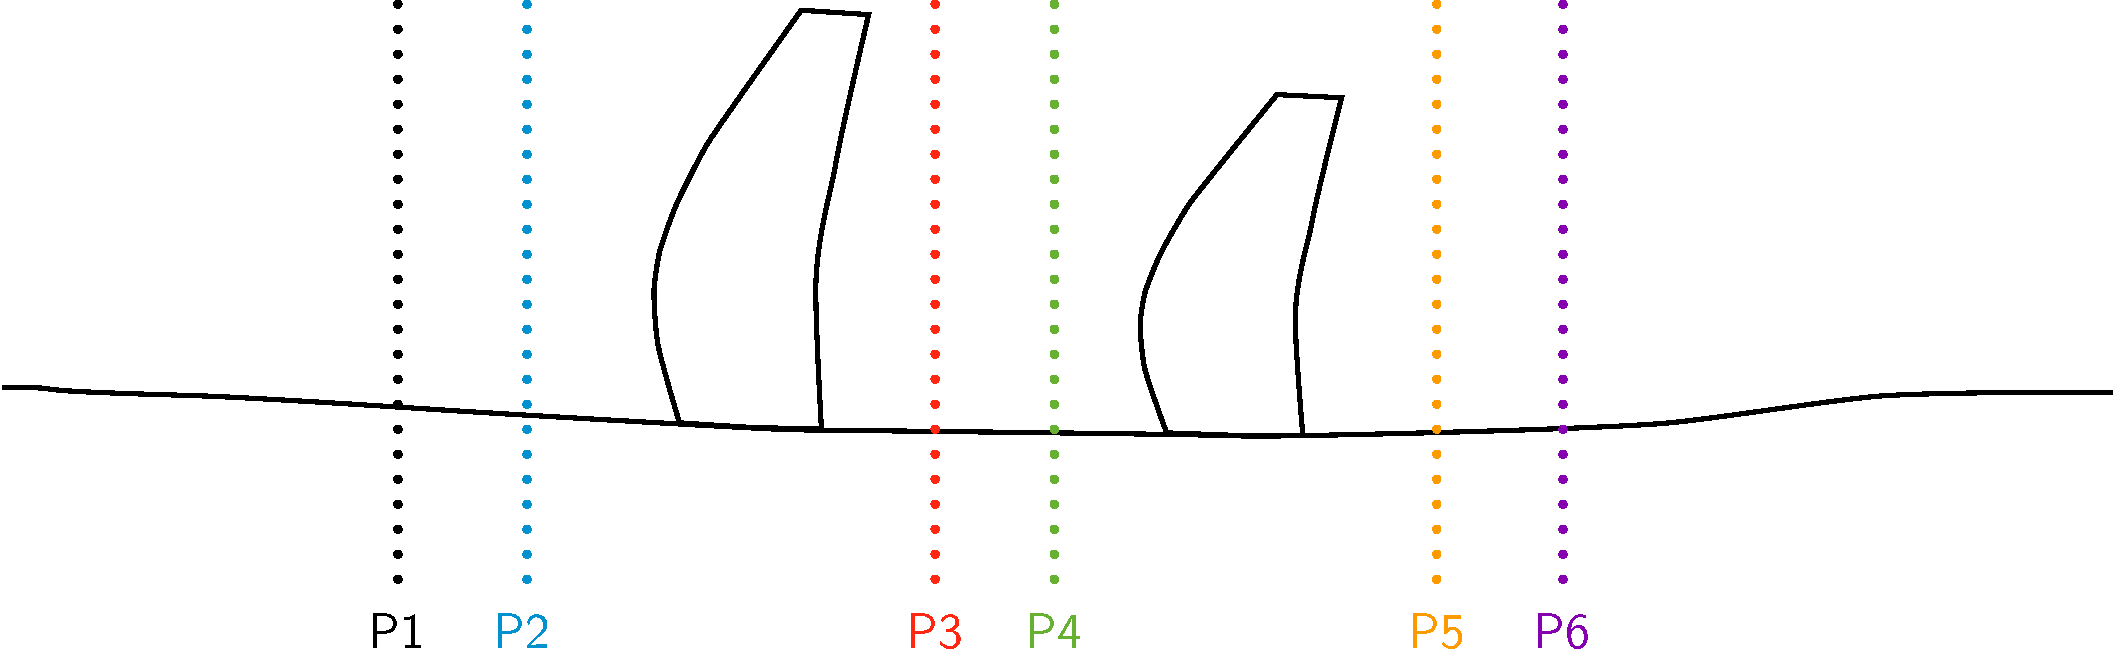
\includegraphics[width=.55\textwidth]{dream_position_azi_mean.pdf}}
  \subfigure[absolute Mach number]{
    \label{fig:dream_ls_radial_profiles_ma}
    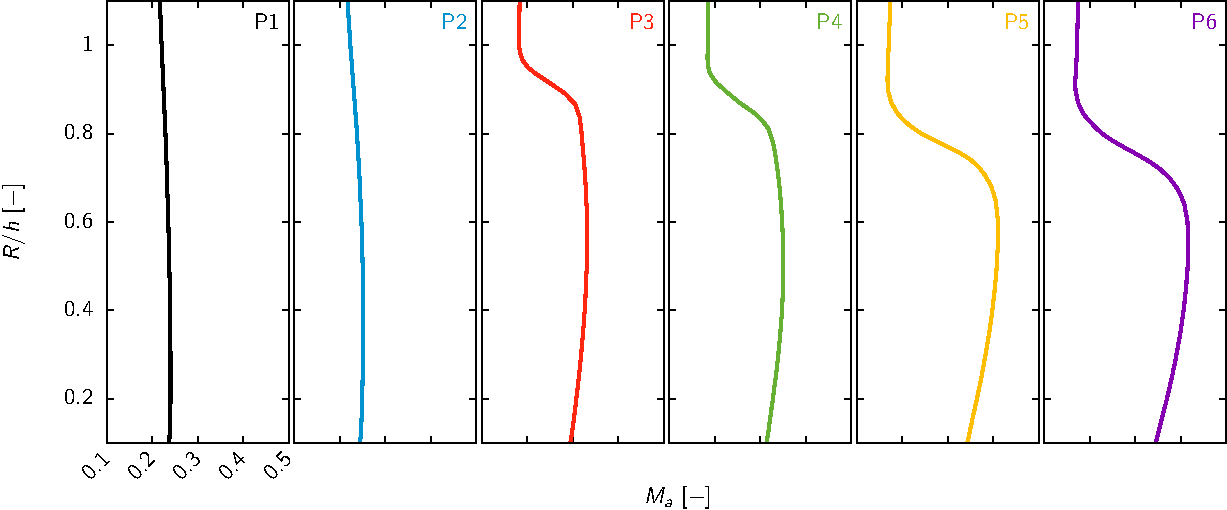
\includegraphics[width=.72\textwidth]{DREAM_LS_RANS_AZI_MEAN_PPT_macha.pdf}}
  \subfigure[absolute flow angle]{
    \label{fig:dream_ls_radial_profiles_alpha}
    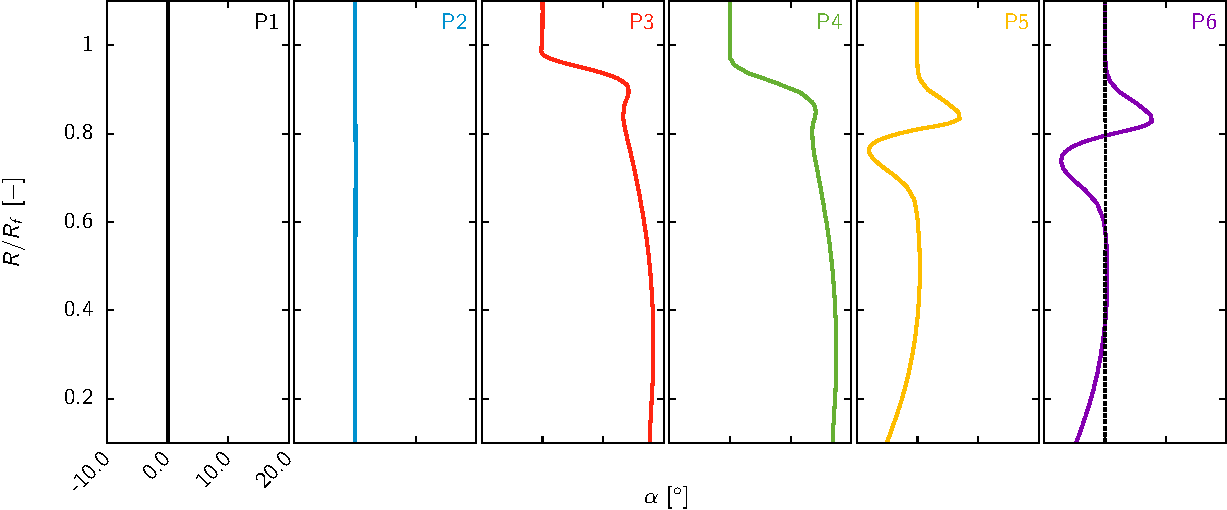
\includegraphics[width=.72\textwidth]{DREAM_LS_RANS_AZI_MEAN_PPT_alpha.pdf}}
  \caption{Low-speed isolated configuration: radial profiles.}
\end{figure}
\setcounter{figure}{\value{figure}-1}
\begin{figure}[htp]
  \centering
  \setcounter{subfigure}{3}
  \subfigure[static pressure]{
    \label{fig:dream_ls_radial_profiles_ps}
    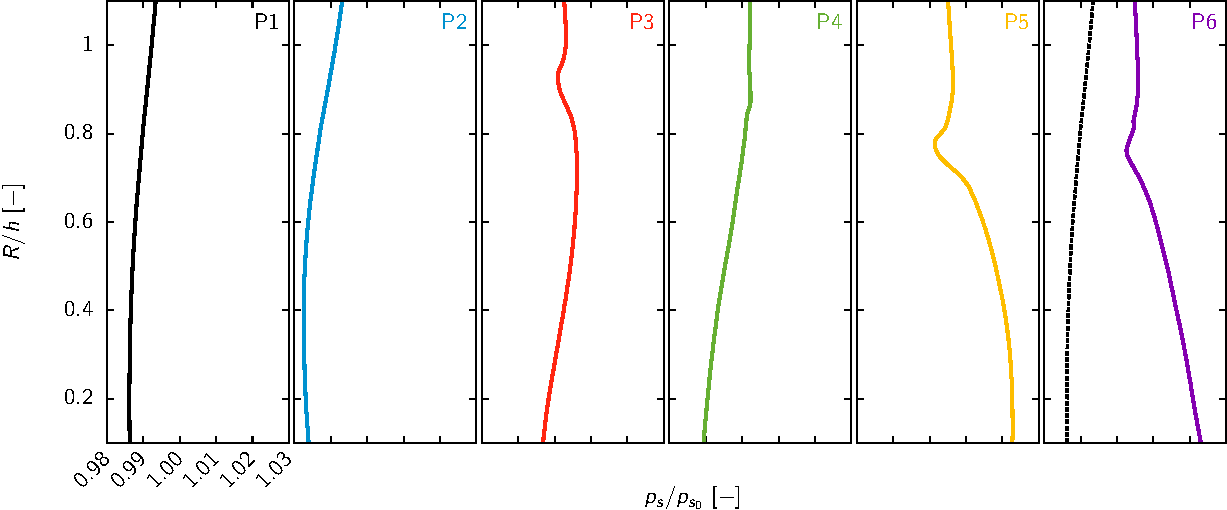
\includegraphics[width=.72\textwidth]{DREAM_LS_RANS_AZI_MEAN_PPT_ps.pdf}}
  \subfigure[stagnation pressure]{
    \label{fig:dream_ls_radial_profiles_pi}
    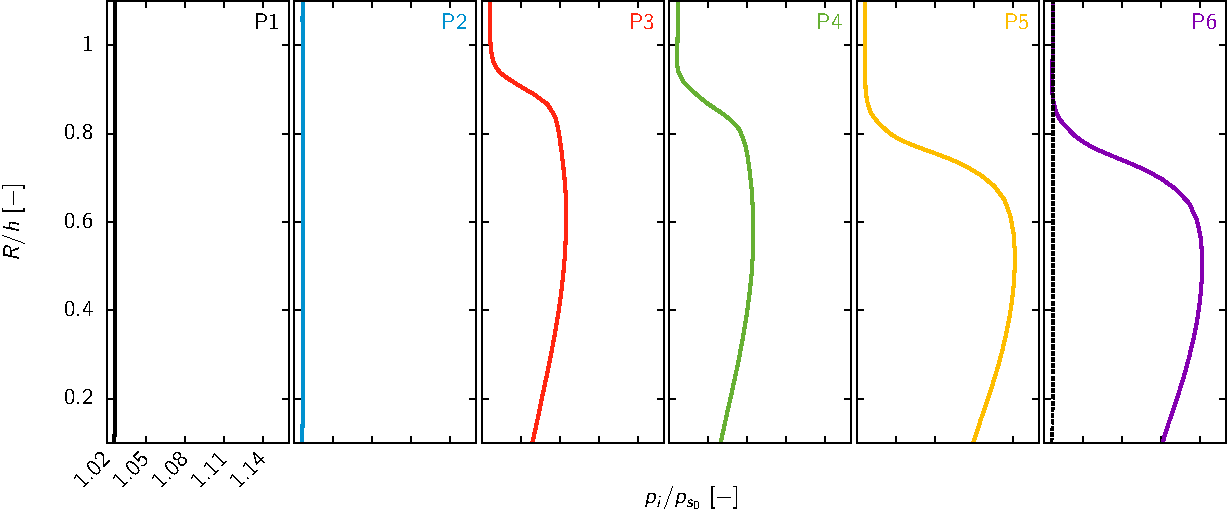
\includegraphics[width=.72\textwidth]{DREAM_LS_RANS_AZI_MEAN_PPT_pi.pdf}}
  \subfigure[stagnation temperature]{
    \label{fig:dream_ls_radial_profiles_ti}
    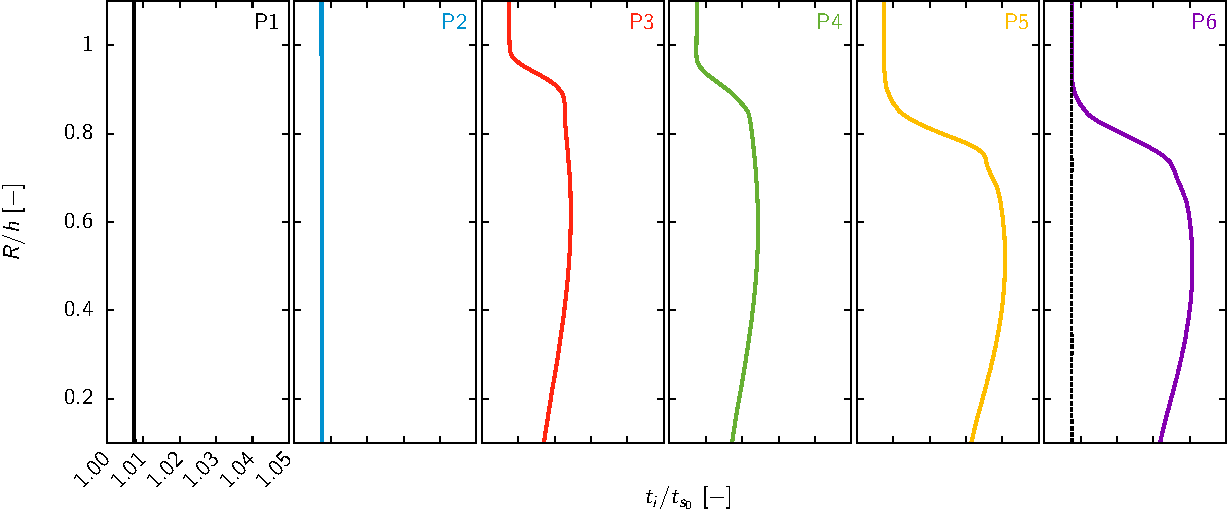
\includegraphics[width=.72\textwidth]{DREAM_LS_RANS_AZI_MEAN_PPT_ti.pdf}}
  \caption{Low-speed isolated configuration: radial profiles (contd.).}
  \label{fig:dream_ls_radial_profiles}
\end{figure}

These 1D results provide us confidence in our simulation. 
In fact, the flow physic that
was expected is observed in the results. To further analyze the simulation,
2D results are presented in the following section.

\subsection{Two dimensional results: radial and axial cuts}
\label{sub:dream_ls_flow_field}

Contours of the relative Mach number are shown in 
Fig.~\ref{fig:dream_ls_mach_kp} along with the pressure coefficient $k_p$,
for both the front and the rear rotor, defined as:
\begin{equation}
   -k_p = - \frac{p_s - p_{s_0}}{\rho n^2 D^2},
\end{equation}
where the $n$ and $D$ parameters are the one of the front rotor
to ease the comparison.

The $- k_p$ should be interpreted as follow, an increasing $- k_p$
means that the pressure gradient is negative, namely the flow
is accelerating. Therefore, the positive  $-k_p$ range is attributed
to the suction side and the negative to the pressure side.
The stagnation point is highlighted
by the minimum of the pressure coefficient. On the pressure side 
($-k_p < 0$) the flow accelerates
toward the trailing edge with a favorable pressure gradient. 
On the suction side, a rapid acceleration of the fluid
is observed near the leading edge 
($\partial (-k_p) / \partial x \gg 0$) followed by
a deceleration of the fluid along with an
adverse pressure gradient.
On the front rotor, the integrated pressure coefficient is
increasing along with the relative span, at least 
when comparing the 50~\% and the 75~\% relative spans.
After that, the pressure coefficient is almost constant on 
the front rotor. The loading is thus almost constant for
relative spans greater than 50~\%. In the propeller community and
by extension the CROR community, the loading of a blade is known
to be maximal for a relative span of 75~\%~\cite{Bousquet2012},
which is consistent with our results.

The pressure coefficients on the rear rotor have a similar shape
compared to the one of the front rotor. However, the loading is
larger on the rear rotor and near the tip of the blade
$R/R_f > 75~\%$, the integrated value of the pressure coefficient
increases drastically. This is highlighted by the thrust coefficient 
of the rear rotor $C_{T_f}$ which is reported in 
Tab.~\ref{tab:dream_ls_sim_coeff} and that is higher than
the front rotor one. This is observed even though the diameter of the front
rotor is chosen to normalize the pressure coefficient which
lessened the thrust coefficient of the rear rotor.

Relative Mach number contours are also shown in 
Fig.~\ref{fig:dream_ls_mach_kp}.
As inferred by the tip Mach number value $M_{tip}$ of the blade
given in Tab.~\ref{tab:dream_ls_flight_condition},
the relative Mach number does not 
cross the sonic boundary $M_{rel} = 1$.
The flow remains subsonic which is, aerodynamically speaking,
a good feature for the performances since shocks create losses.
Near the tip region of the rear rotor blades, the leaving of
the tip vortex can be seen. For relative span $R/R_f > 75\%$,
a large low velocity region is seen on the rear rotor blades.
This is due to the strong loading of the rear rotor blades.
\begin{figure}[htp]
 \centering
 \begin{tabular}{rccc}
   & $-k_p$ front rotor
   & $-k_p$ rear rotor
   & relative Mach number\\
   \rotatebox{90}{\qquad\qquad 25~\%} 
   & 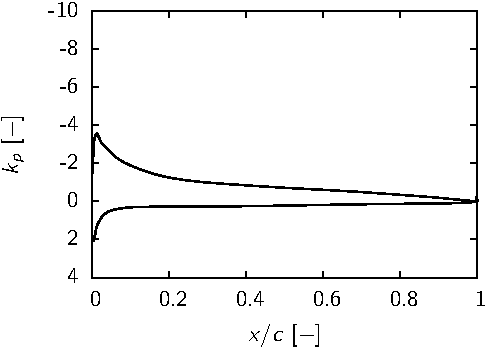
\includegraphics[width=0.28\textwidth]{DREAM_LS_KP_25_FRONT_PPT.pdf}
   & 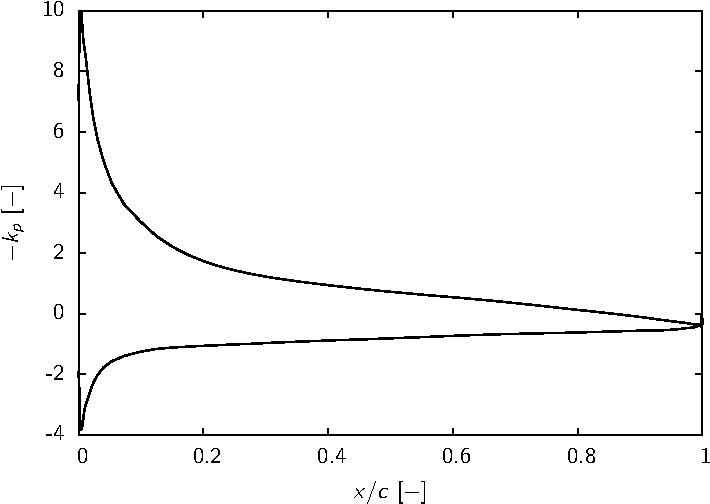
\includegraphics[width=0.28\textwidth]{DREAM_LS_KP_25_REAR_PPT.pdf}
   & 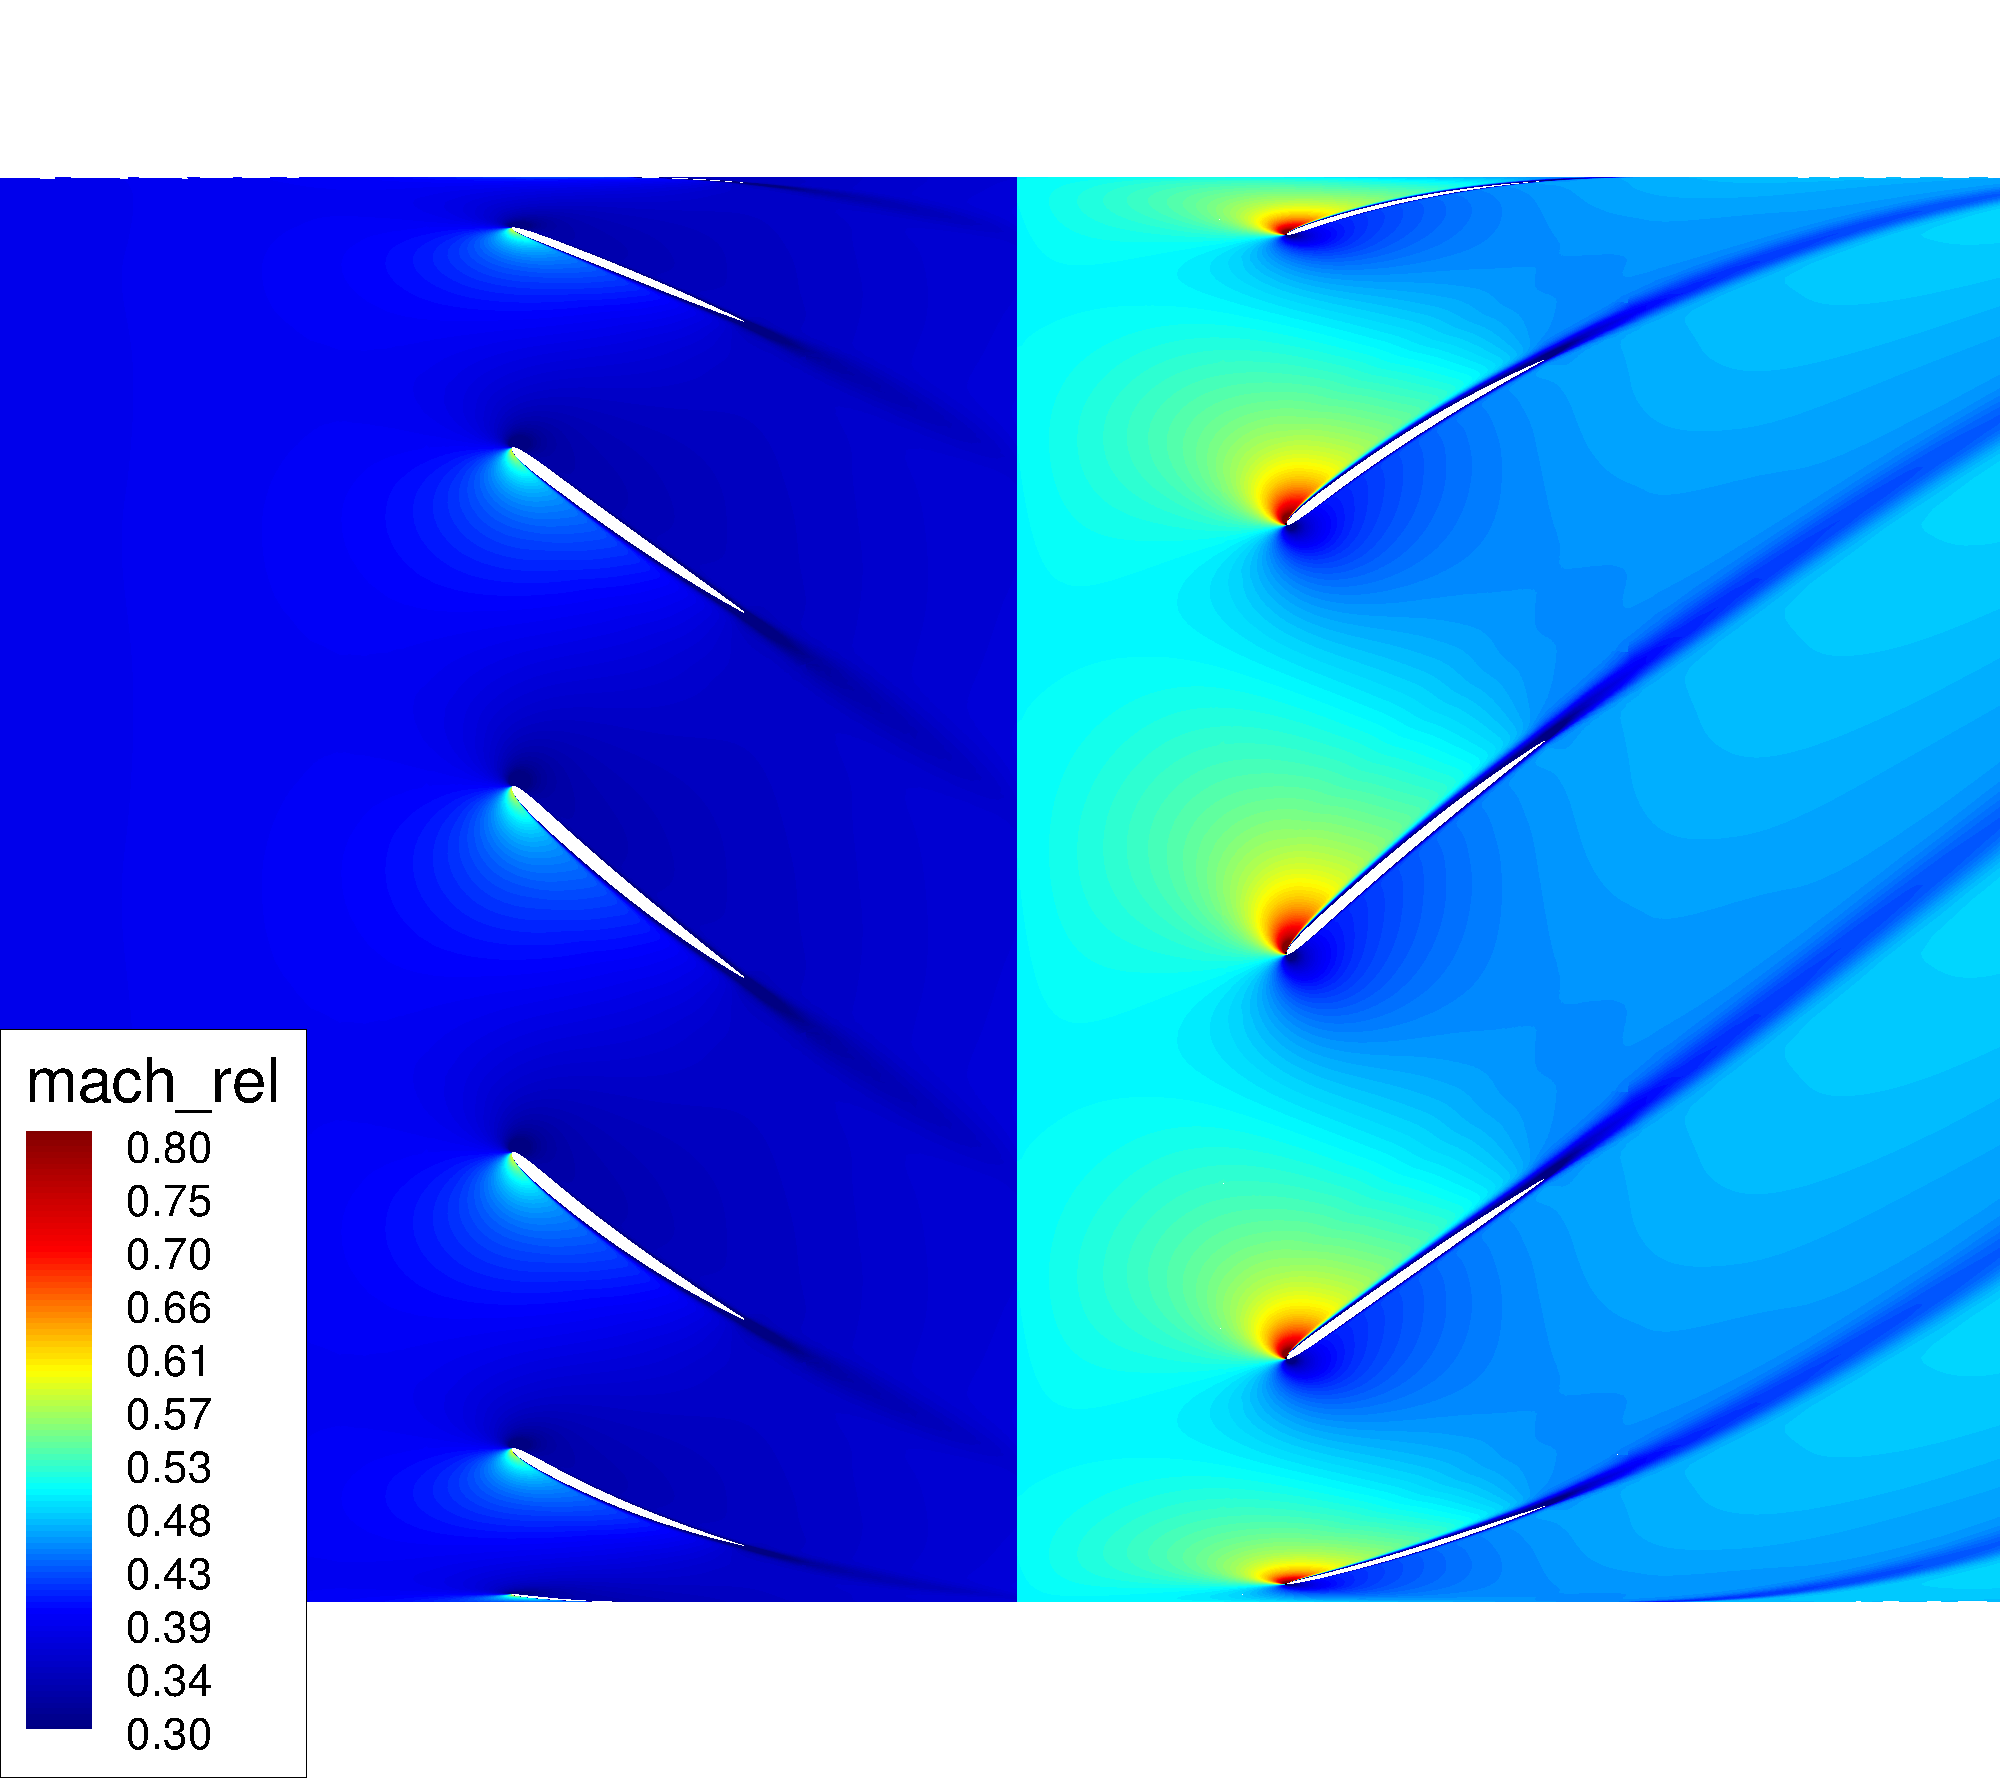
\includegraphics[width=0.28\textwidth]{DREAM_LS_RANS_roe2_sa_slice_r_25_mach_rel.png}\\
   \rotatebox{90}{\qquad\qquad 50~\%} 
   & 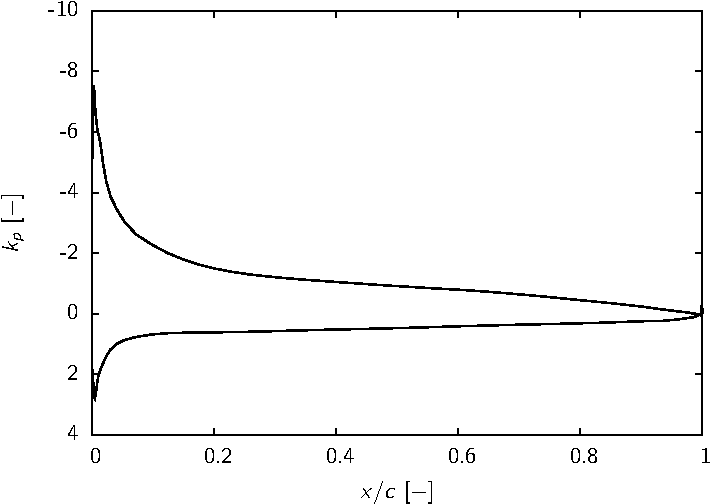
\includegraphics[width=0.28\textwidth]{DREAM_LS_KP_50_FRONT_PPT.pdf}
   & 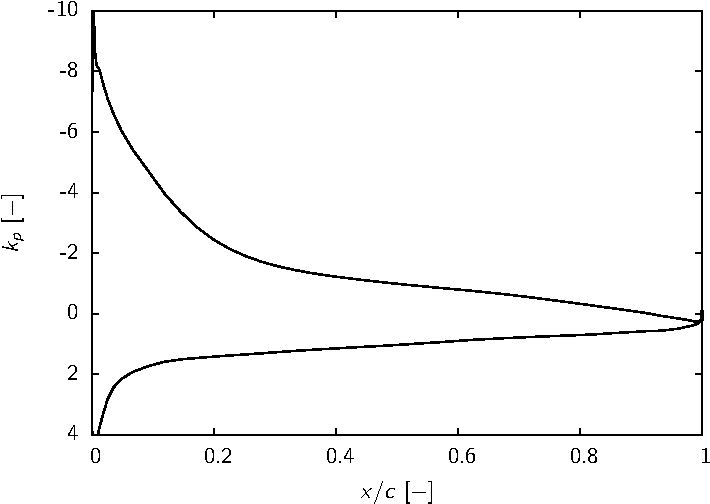
\includegraphics[width=0.28\textwidth]{DREAM_LS_KP_50_REAR_PPT.pdf}
   & 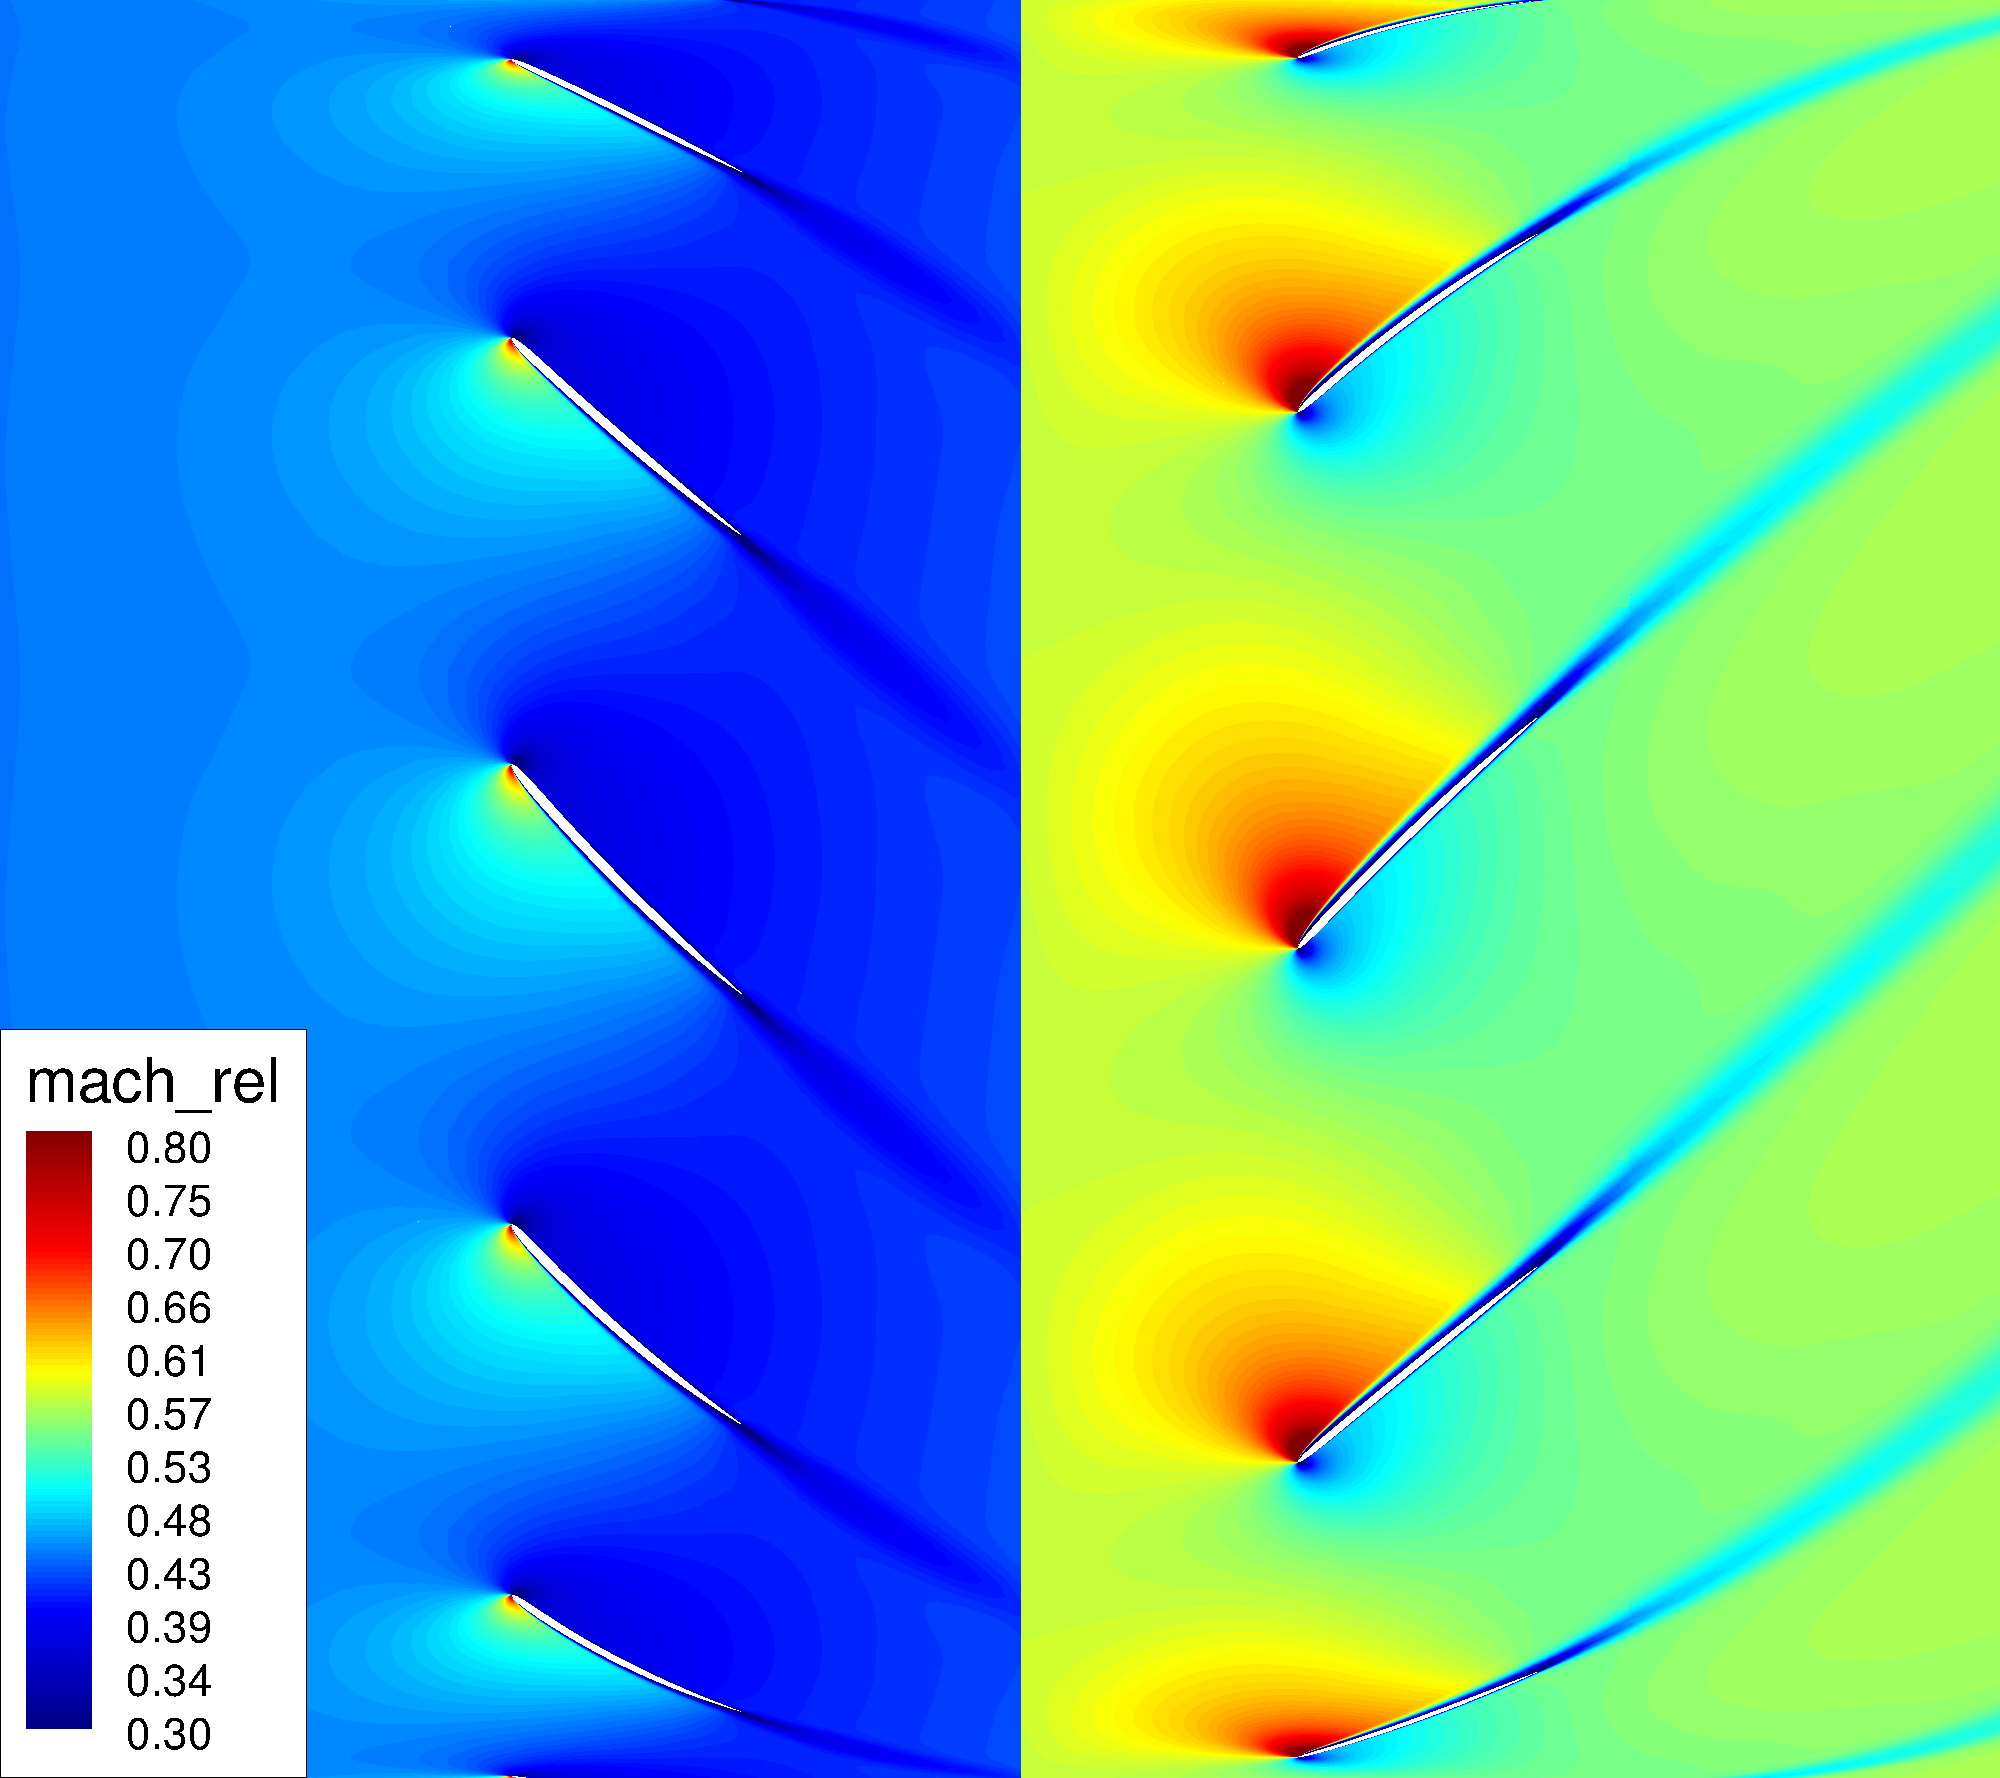
\includegraphics[width=0.28\textwidth]{DREAM_LS_RANS_roe2_sa_slice_r_50_mach_rel.png}\\
   \rotatebox{90}{\qquad\qquad 75~\%} 
   & 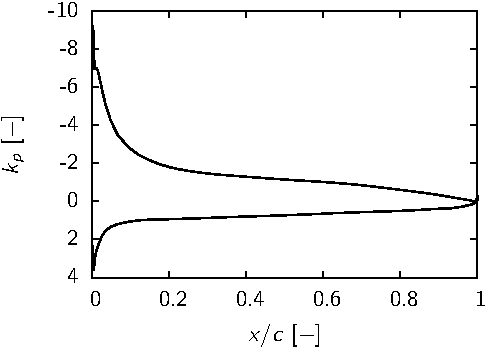
\includegraphics[width=0.28\textwidth]{DREAM_LS_KP_75_FRONT_PPT.pdf}
   & 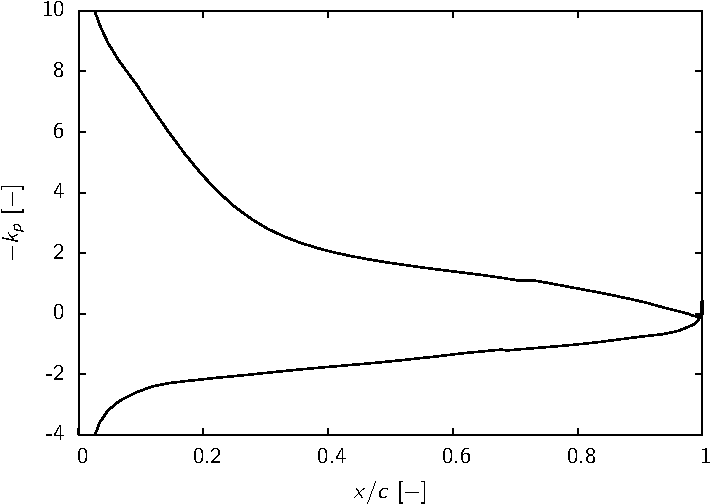
\includegraphics[width=0.28\textwidth]{DREAM_LS_KP_75_REAR_PPT.pdf}
   & 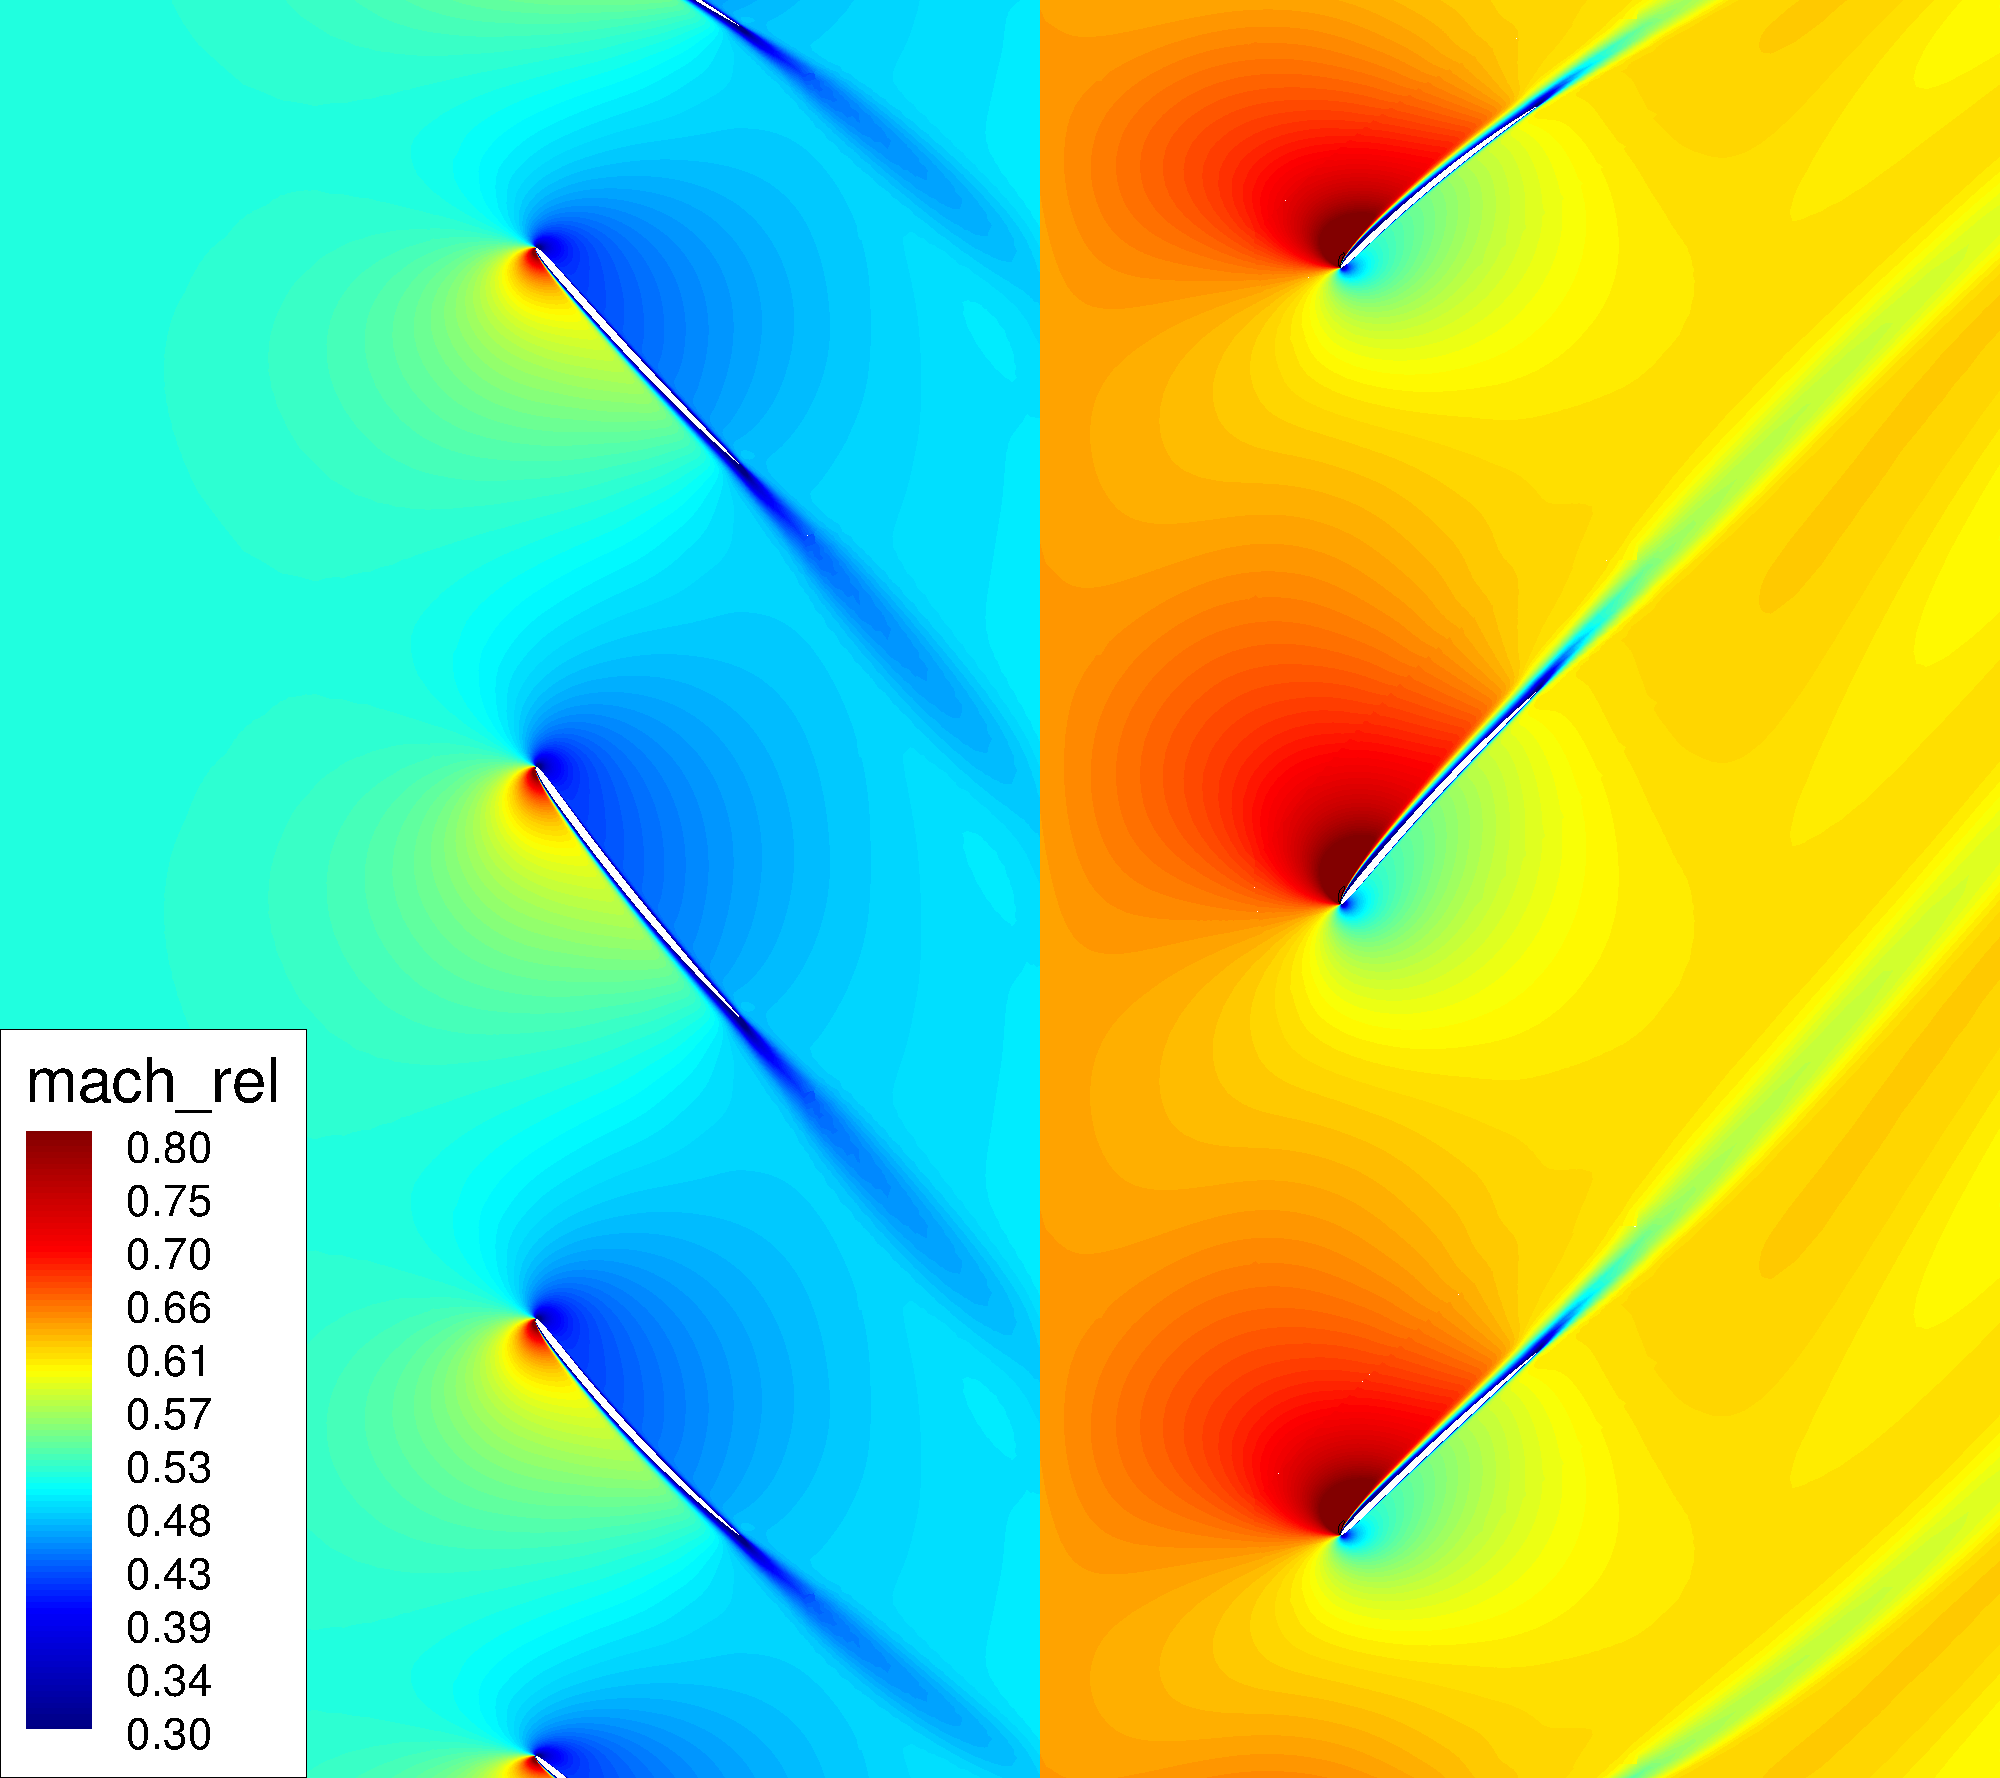
\includegraphics[width=0.28\textwidth]{DREAM_LS_RANS_roe2_sa_slice_r_75_mach_rel.png}\\
   \rotatebox{90}{\qquad\qquad 90~\%} 
   & 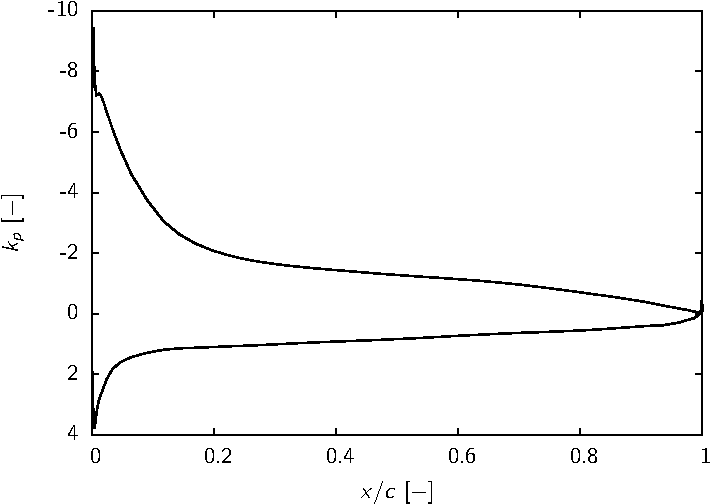
\includegraphics[width=0.28\textwidth]{DREAM_LS_KP_90_FRONT_PPT.pdf}
   & 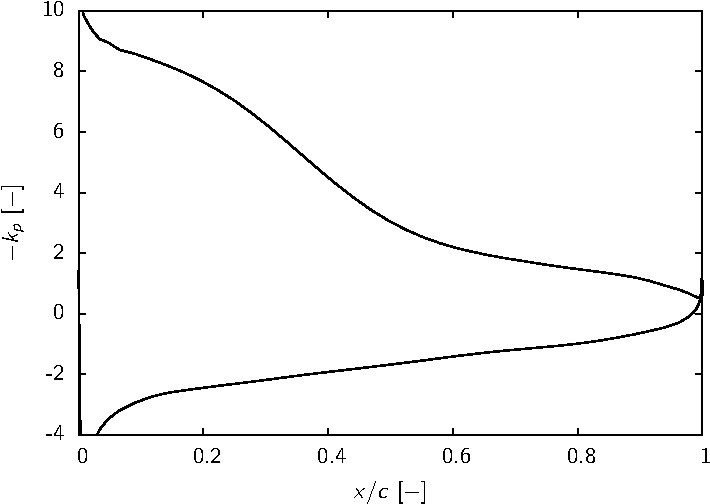
\includegraphics[width=0.28\textwidth]{DREAM_LS_KP_90_REAR_PPT.pdf}
   & 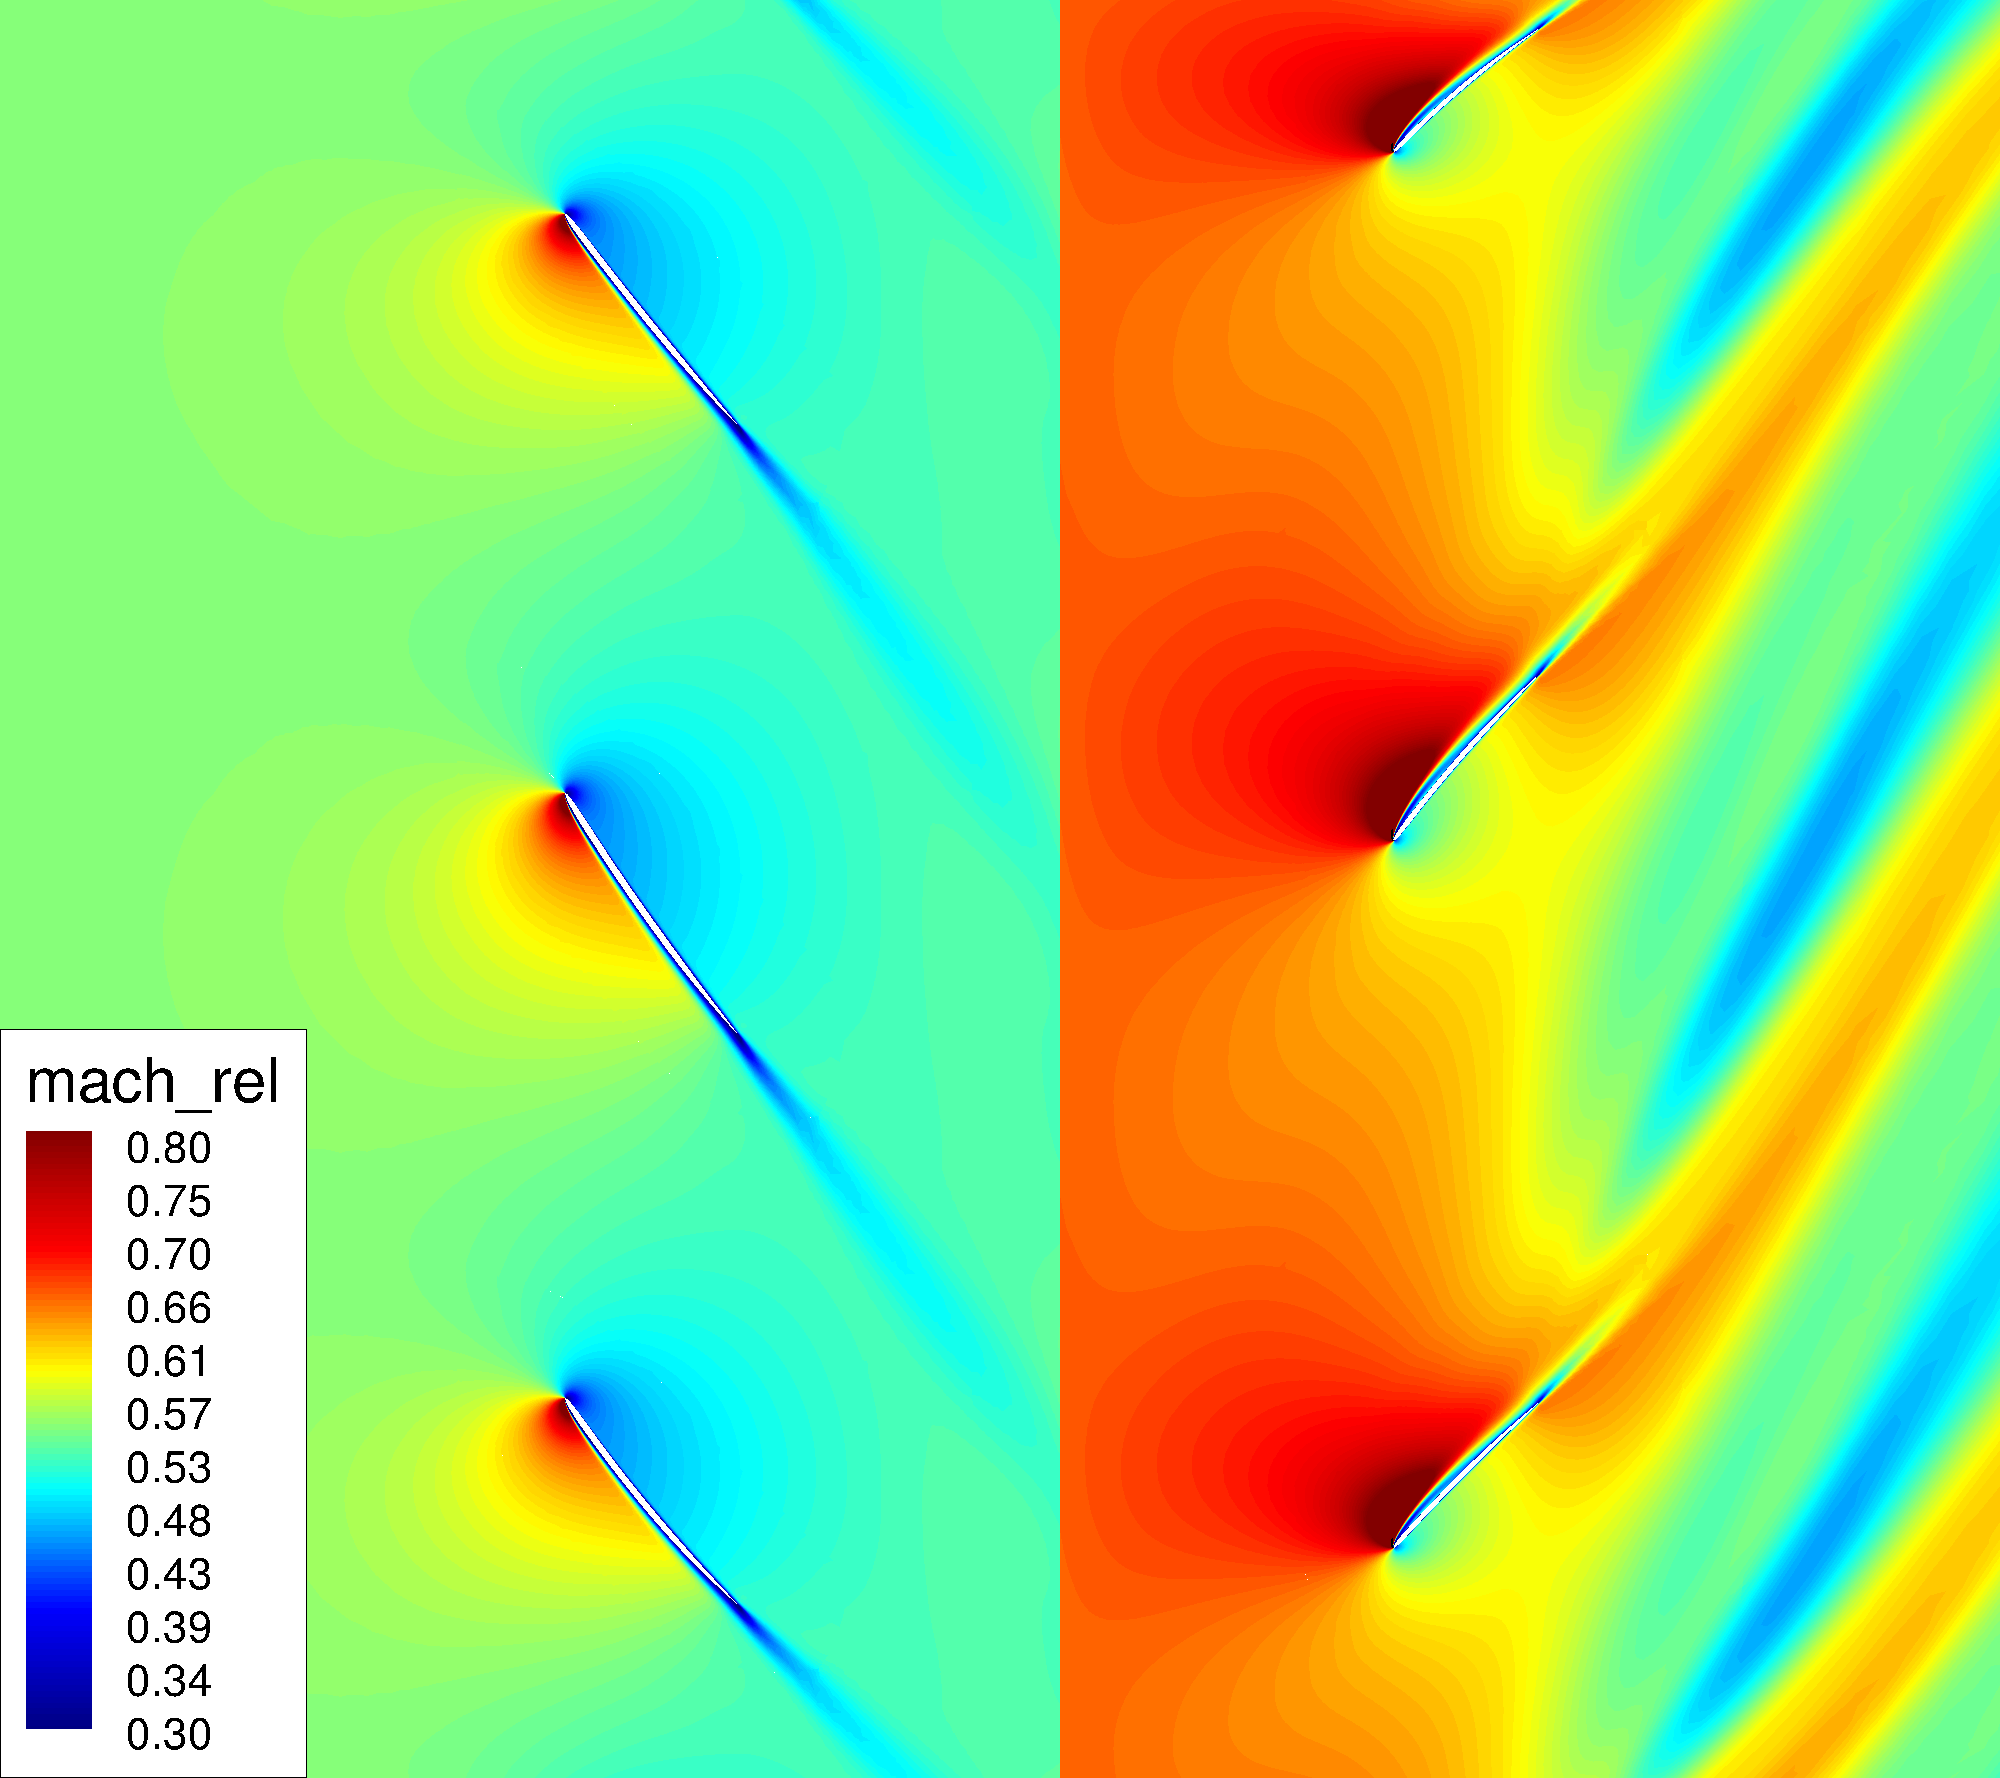
\includegraphics[width=0.28\textwidth]{DREAM_LS_RANS_roe2_sa_slice_r_90_mach_rel.png}\\
   \rotatebox{90}{\qquad\qquad 95~\%} 
   & 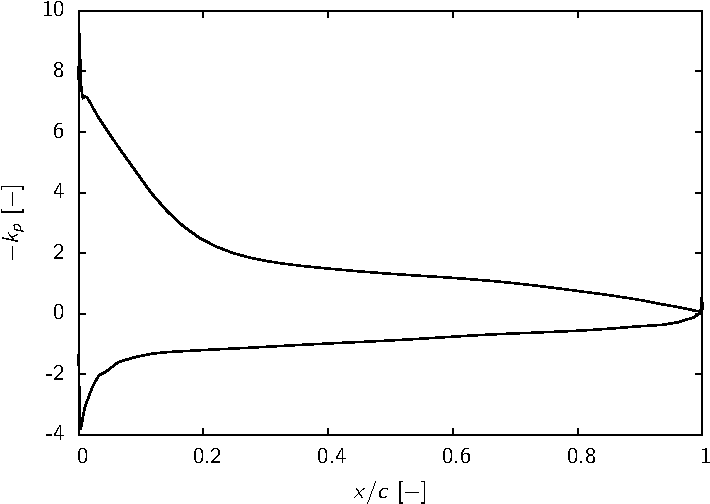
\includegraphics[width=0.28\textwidth]{DREAM_LS_KP_95_FRONT_PPT.pdf}
   & 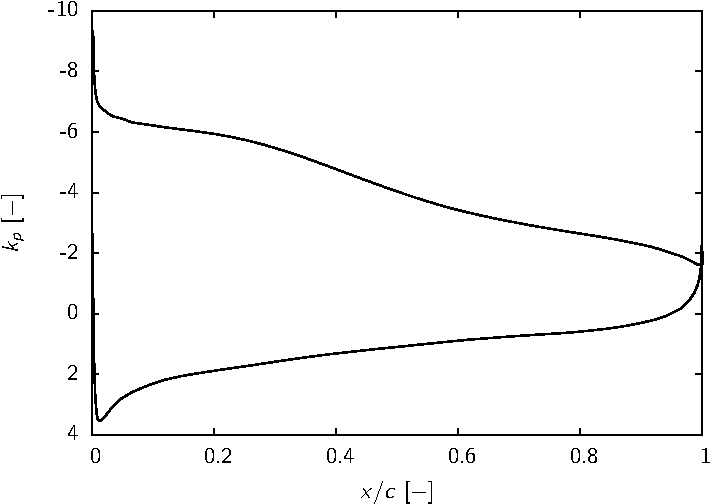
\includegraphics[width=0.28\textwidth]{DREAM_LS_KP_95_REAR_PPT.pdf}
   & 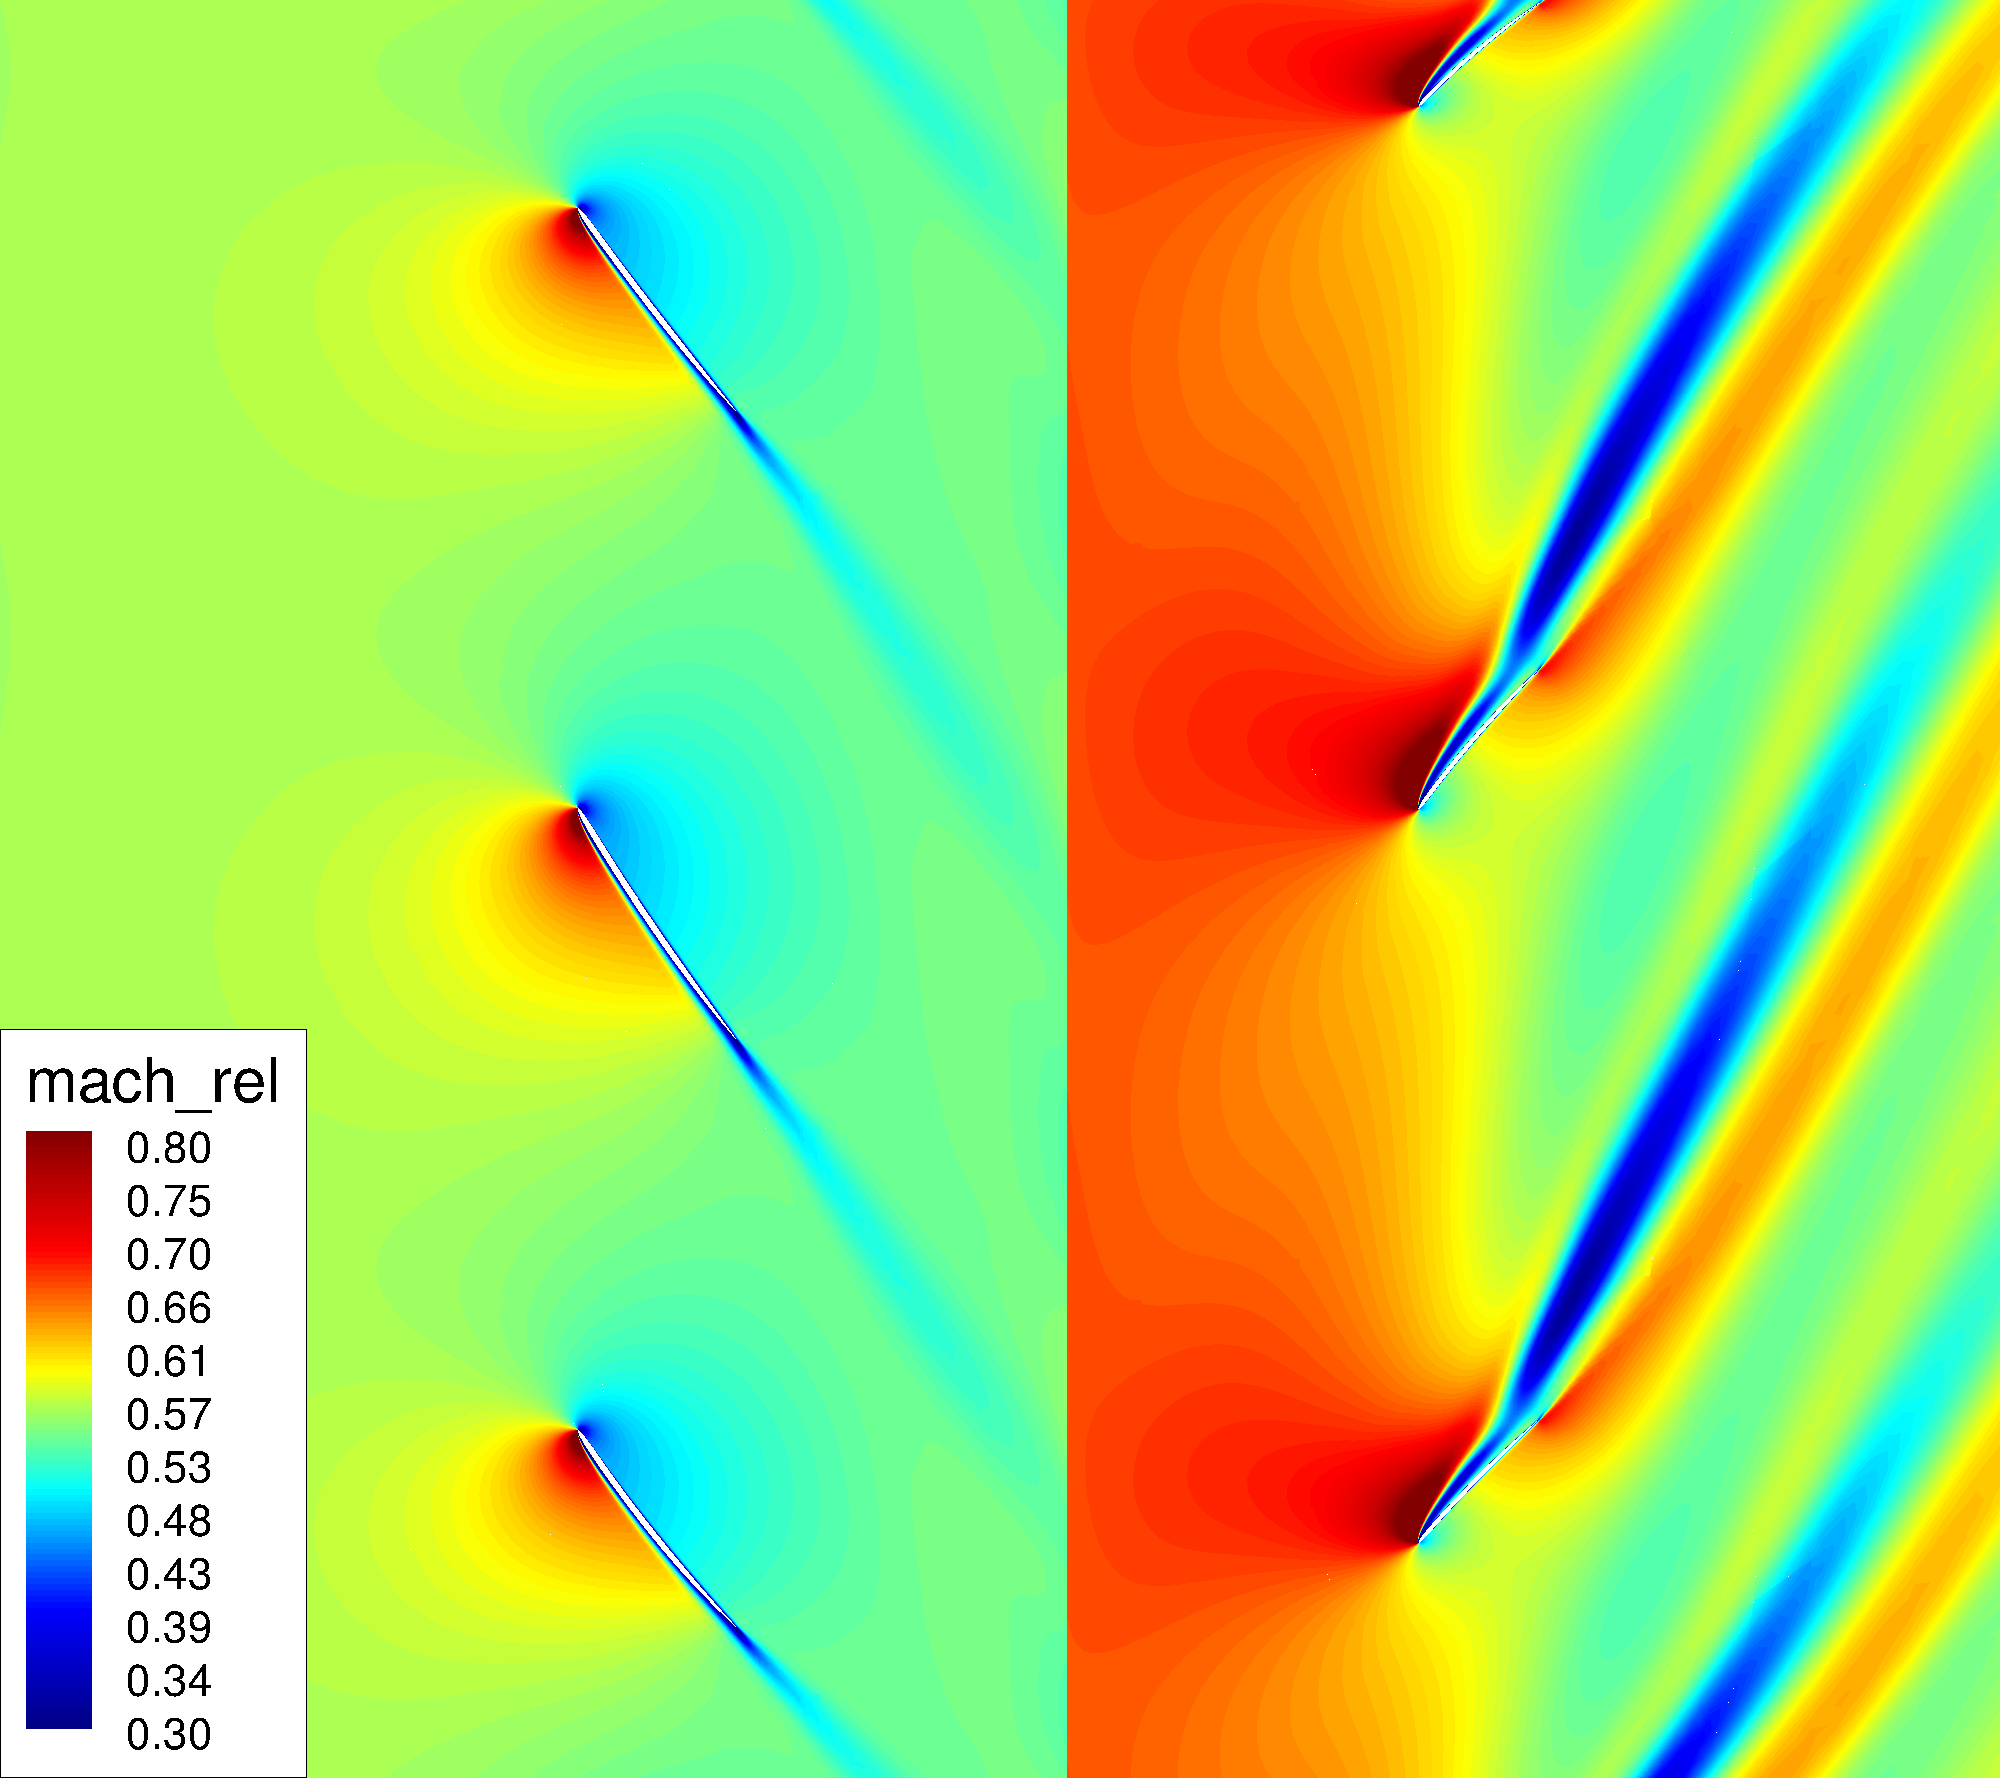
\includegraphics[width=0.28\textwidth]{DREAM_LS_RANS_roe2_sa_slice_r_95_mach_rel.png}  
 \end{tabular}
 \caption{Low-speed isolated configuration: pressure coefficient and relative Mach
 number contours at different radial position.}
 \label{fig:dream_ls_mach_kp}
\end{figure}

Axial cuts of the entropy are shown in Fig.~\ref{fig:dream_ls_steady_entropy}.
The axial positions are the four planes $P3$, $P4$, $P5$
and $P6$ as defined in Fig.~\ref{fig:dream_ls_position_radial}.
The tip vortices generated by the front rotor are seen in the $P3$
axial plane. The mixing plane approach is used for the steady computations
presented here. This is emphasized by the $P4$ axial cut of entropy. A
smooth, spatially-averaged field of entropy is seen with a 
ring of losses attributed to the front rotor tip vortices. This is of course the main
weakness of the steady approach used here to compute the CROR configuration.
In fact, as recalled in Chap.~\ref{cha:cror}, the tip vortices and the wakes shed by the
front rotor blades can impact the rear rotor blades and thus generate
exceeding level of unsteadinesses, responsible for noise and vibration. As the influence
of the front rotor tip vortices is azimuthally-averaged, it is
lessened. Therefore unsteady computations will be needed to
predict the unsteady interactions of the front rotor with the rear one.
This is the aim of the forthcoming Section~\ref{sec:dream_ls_rigid_results}.
The remaining axial planes extracted at $P5$ and $P6$ depict the strong loading
of the rear rotor blades. In fact, baring in mind that the
axial planes are equidistant from the blades, the larger the loss traces,
the stronger the loading of the blades. Moreover, even though the
tip vortices shed by the front rotor 
blades are azimuthally-averaged,
their trace is still seen and seems to indicate that they will
interact with the rear rotor tip vortices.
\begin{figure}[htp]
  \centering
  \subfigure[$P3$]{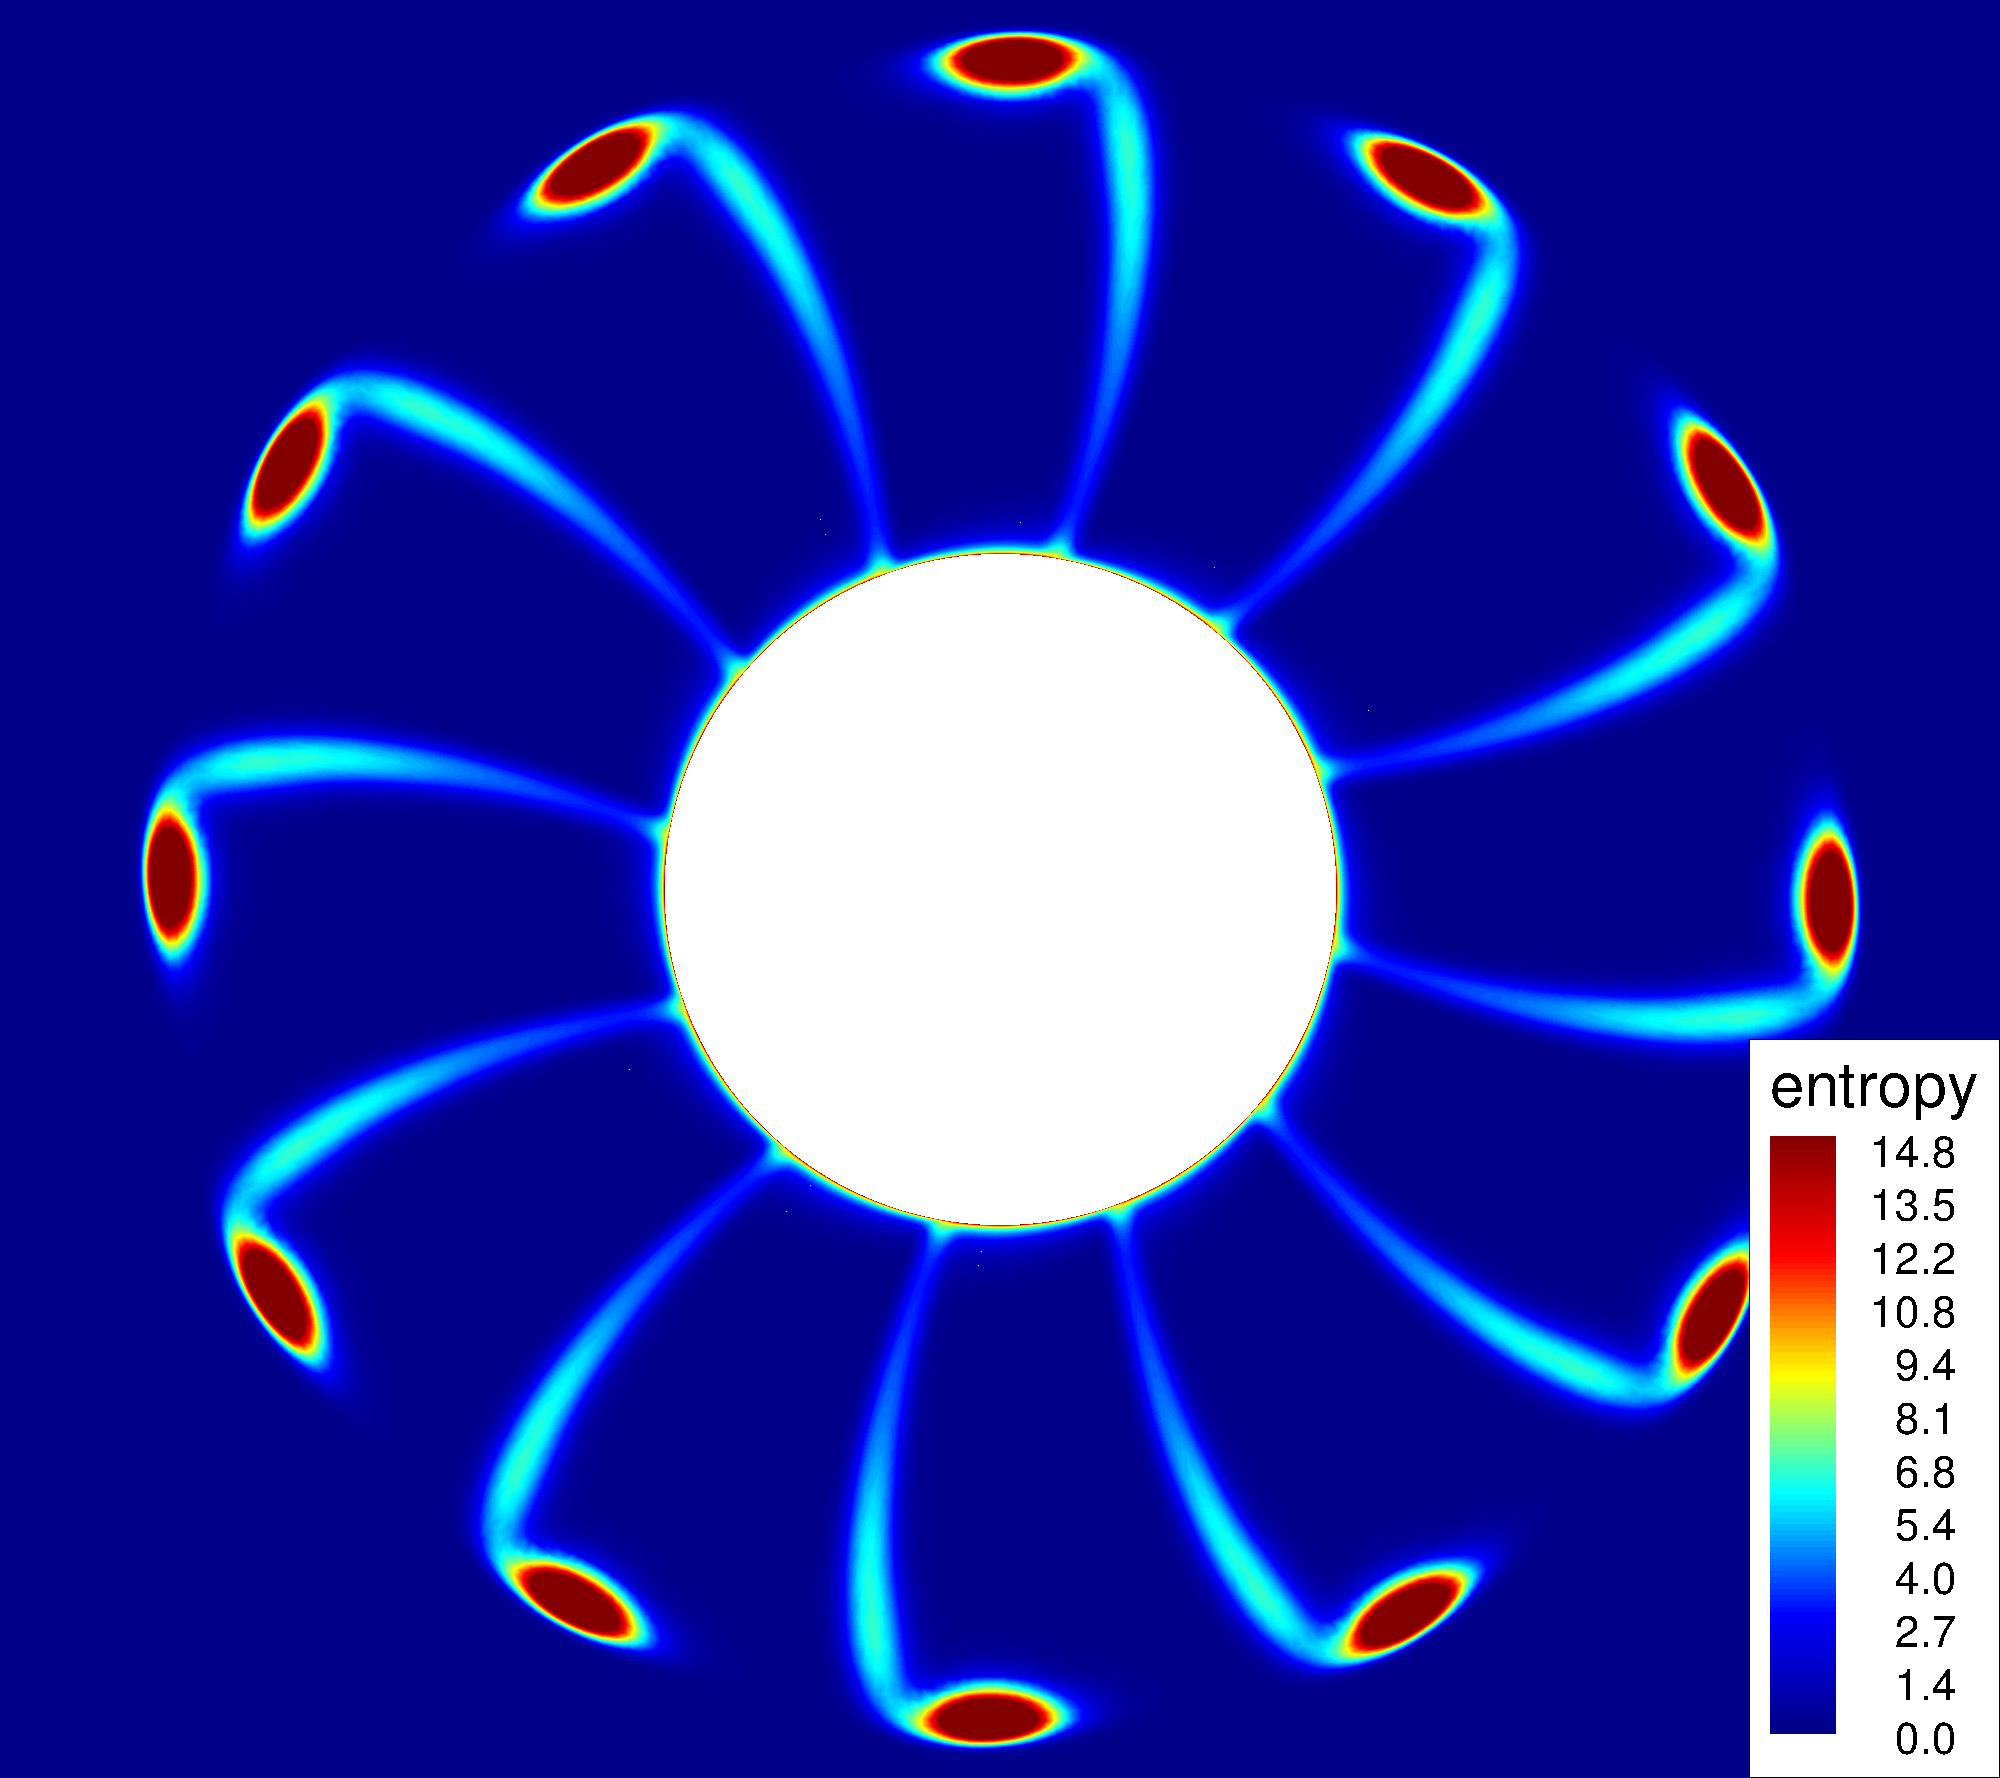
\includegraphics[width=.35\textwidth]{DREAM_LS_RANS_roe2_sa_slice_x_front_1_entropy.png}}
  \subfigure[$P4$]{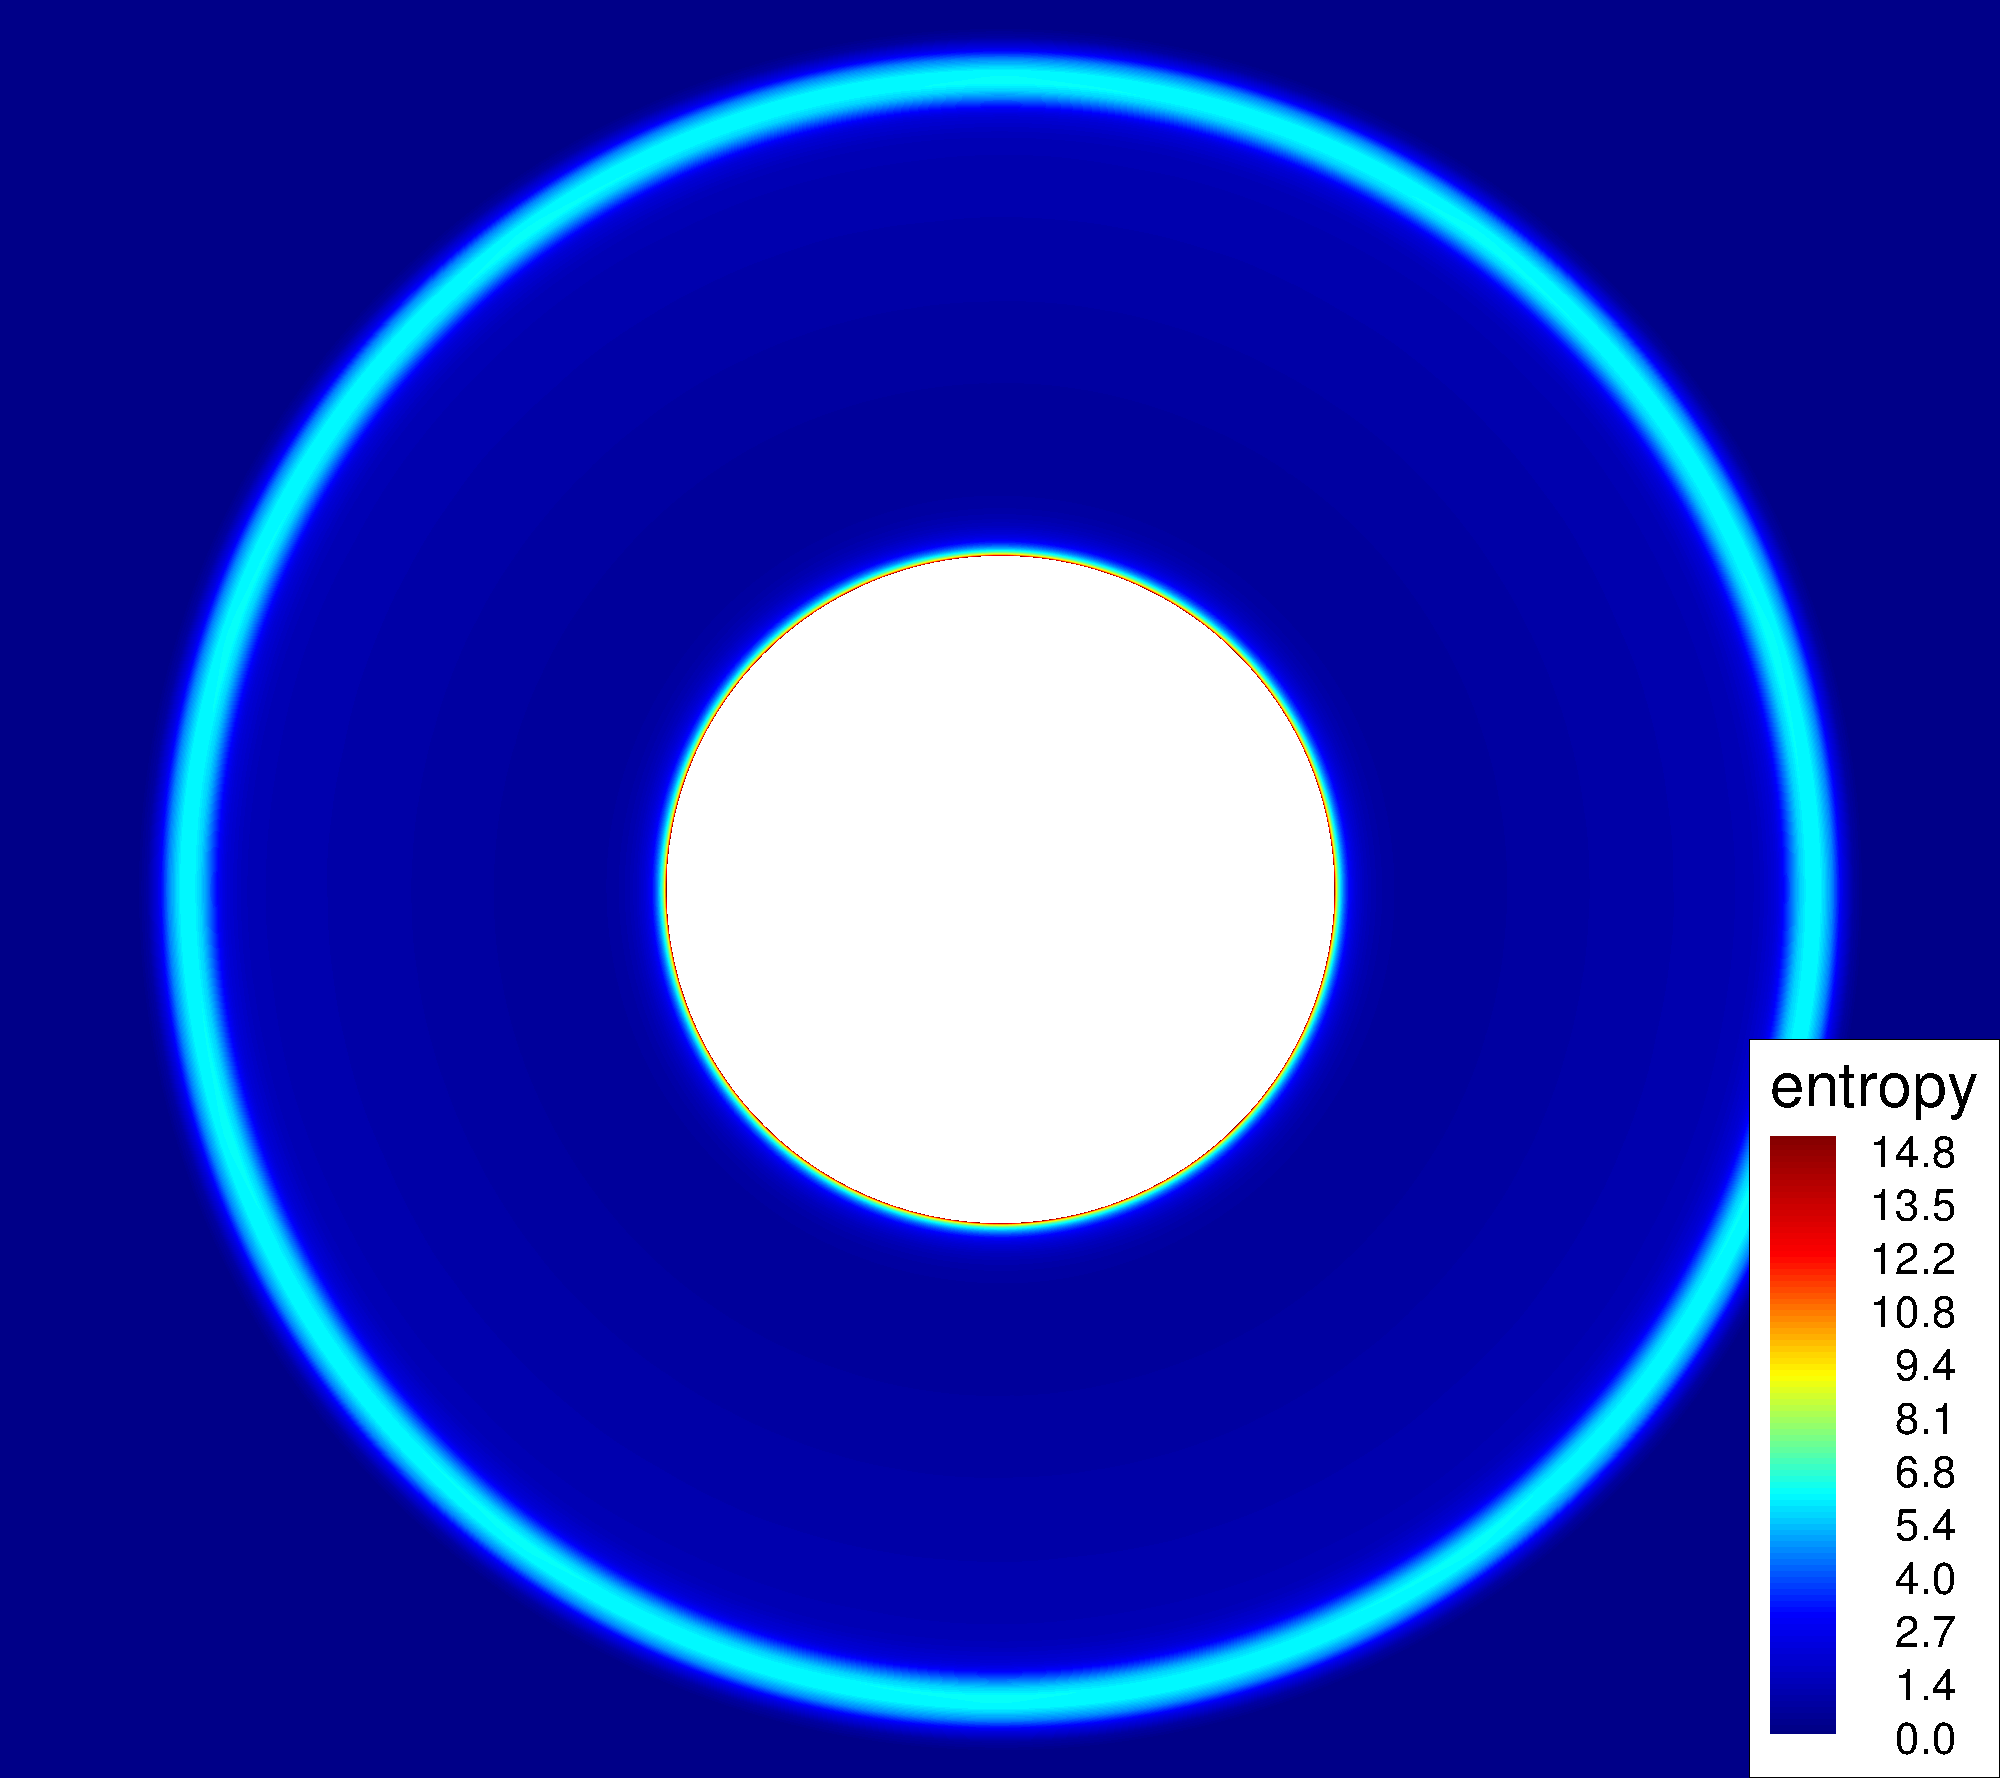
\includegraphics[width=.35\textwidth]{DREAM_LS_RANS_roe2_sa_slice_x_rear_-1_entropy.png}}
  \subfigure[$P5$]{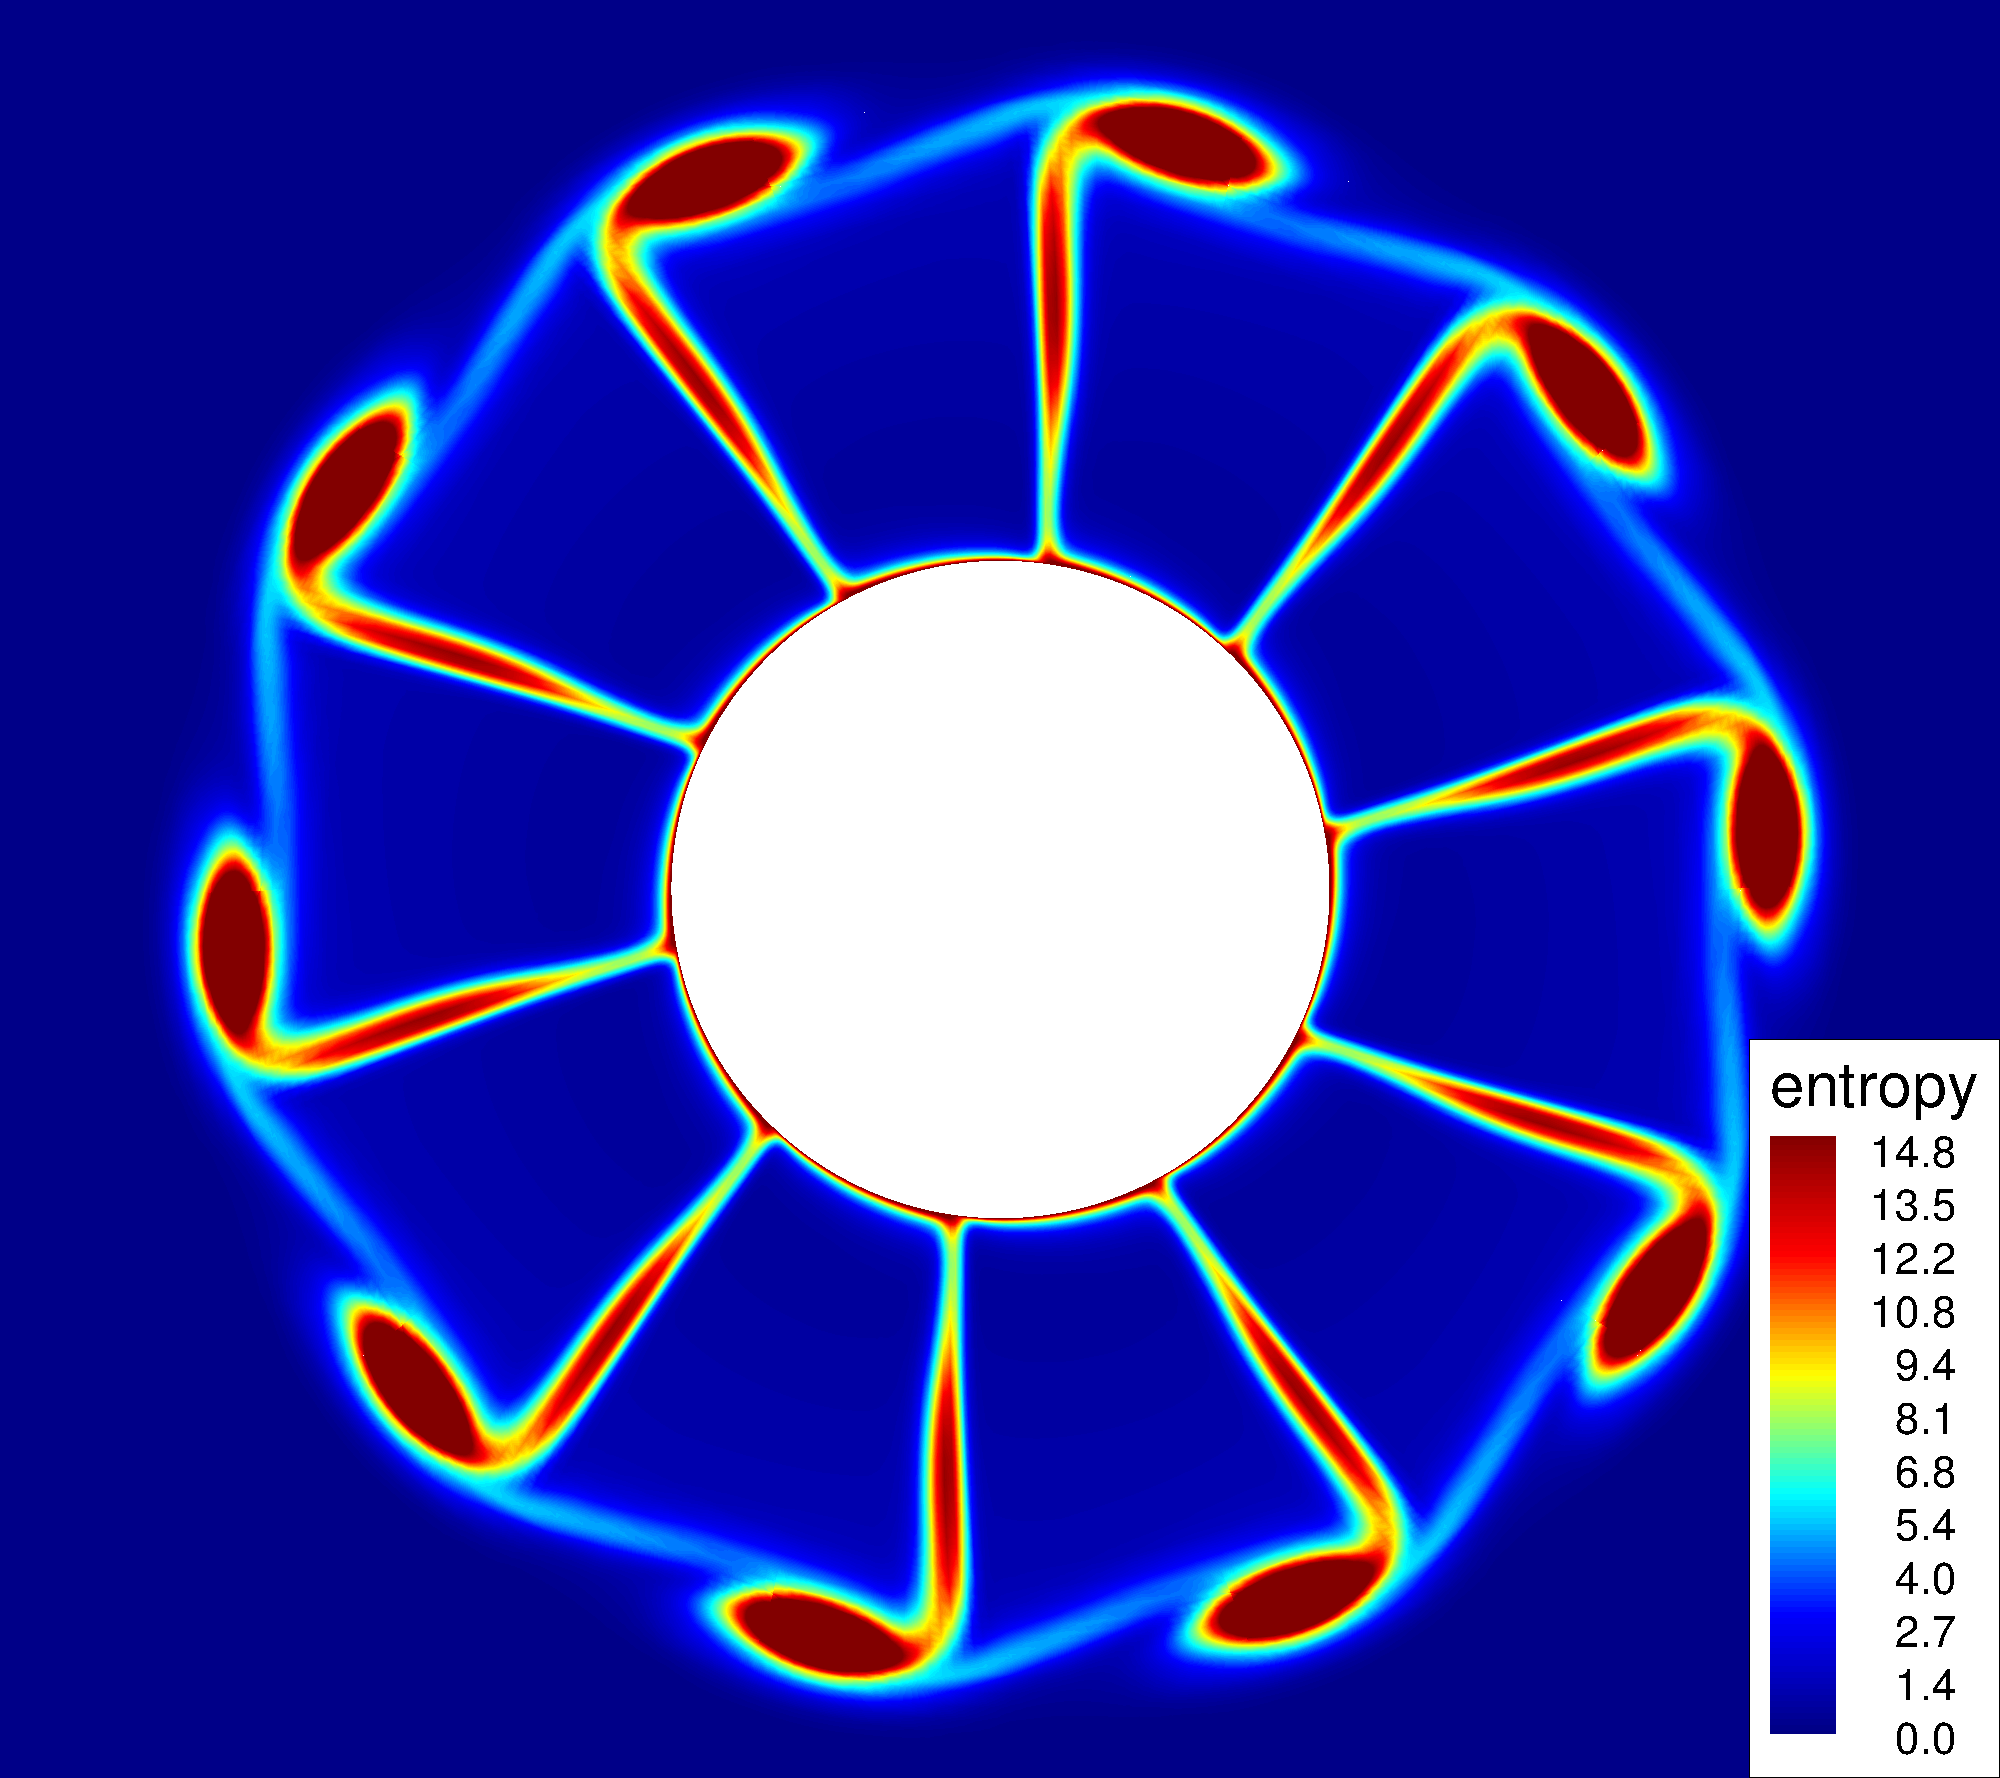
\includegraphics[width=.35\textwidth]{DREAM_LS_RANS_roe2_sa_slice_x_rear_1_entropy.png}}
  \subfigure[$P6$]{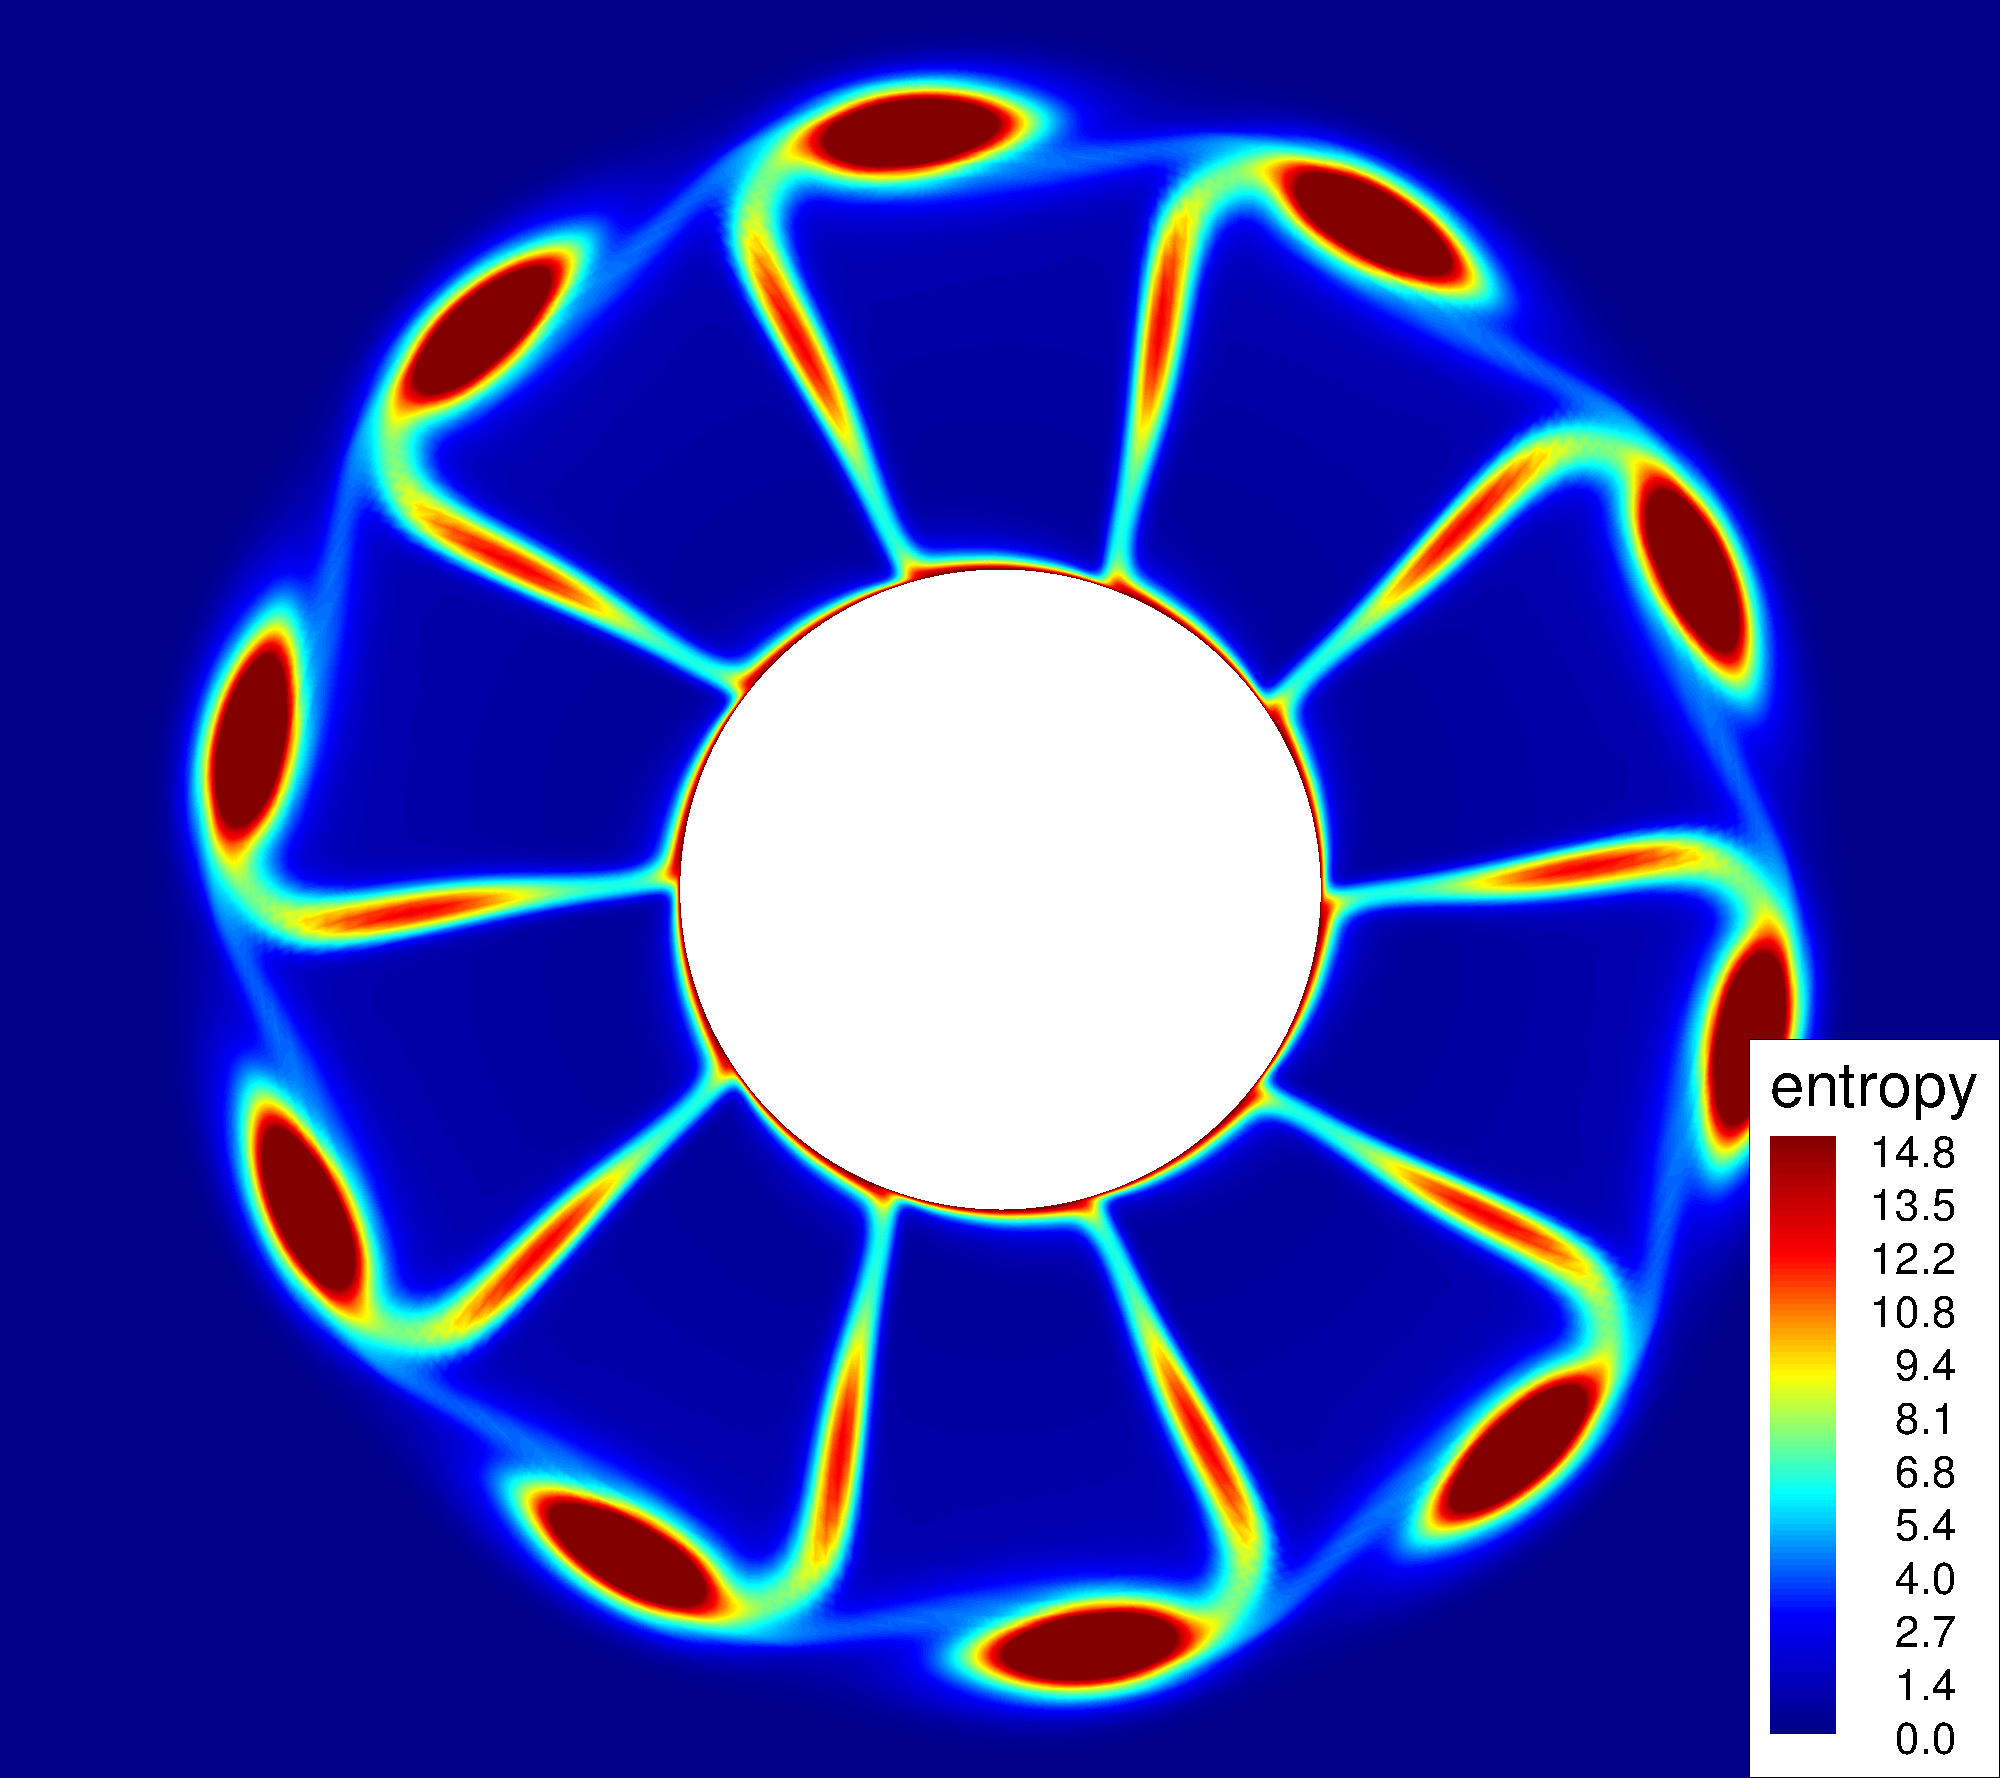
\includegraphics[width=.35\textwidth]{DREAM_LS_RANS_roe2_sa_slice_x_rear_2_entropy.png}}
  \caption{Low-speed isolated configuration: axial cuts of entropy.}
   \label{fig:dream_ls_steady_entropy}
\end{figure}